\documentclass[twoside]{article} \usepackage{aistats2017}



%\usepackage[cmex10]{amsmath, mathtools}
\usepackage{amsmath,amssymb,amsbsy,amsfonts,amsthm}
\usepackage{multirow}
\usepackage{bm}
\usepackage{enumerate}
\usepackage{url}
\usepackage[ruled,vlined]{algorithm2e}
\usepackage{fancyvrb}
\usepackage{yfonts}

\usepackage{wrapfig}
\usepackage{tikz}
%\input{../tikz.conf}

\usetikzlibrary{bayesnet}

%%%%%%%%%%% Box 
\usepackage{calc}%    For the \widthof macro
\usepackage{xparse}%  For \NewDocumentCommand
\newcommand{\tikzmark}[1]{\tikz[overlay,remember picture] \node (#1) {};}


%% Variable de compilation
\newif\ifbeamer
\beamerfalse
\newcommand{\beamer}[2]{\ifbeamer #1 \else #2 \fi}
%%%

%\usepackage[latin1]{inputenc}
\usepackage[utf8]{inputenc} % manage utf8 encodage 
%\usepackage[english]{babel} % for french document ! dirty enumerate style,+ bad change rectangle colors for section linking.
\usepackage{fancyhdr} % for heading
\usepackage{listings}
\usepackage[colorlinks=true, urlcolor=blue]{hyperref} % url, link
\usepackage{graphicx}
\usepackage{geometry}

%\usepackage[cmex10]{amsmath, mathtools}
\usepackage{amsmath,amssymb,amsbsy,amsfonts,amsthm}
\usepackage{multirow}
\usepackage{bm}
\usepackage{enumerate}
\usepackage{url}
\usepackage[ruled,vlined]{algorithm2e}
\usepackage{fancyvrb}
\usepackage{yfonts}

\usepackage{wrapfig}
\usepackage{tikz}
    %\input{../tikz.conf}
    
\usetikzlibrary{bayesnet}
    
%%%%%%%%%%% Box 
\usepackage{calc}%    For the \widthof macro
\usepackage{xparse}%  For \NewDocumentCommand
\newcommand{\tikzmark}[1]{\tikz[overlay,remember picture] \node (#1) {};}

%%%%%%%%%% Math
\renewcommand{\text}{\textnormal}
\newcommand{\pr}{\mathbf{p}}
\newcommand{\E}{\mathbb{E}}
\newcommand{\divkk}{\mathbb{K}}
\newcommand{\entropy}{\mathbb{H}}
\newcommand{\gem}{\mathrm{GEM}}
\newcommand{\Mult}{\mathrm{Mult}}
\newcommand{\DP}{\mathrm{DP}}
\newcommand{\IBP}{\mathrm{IBP}}
\newcommand{\M}{\mathcal{M}}
\newcommand{\V}{\mathcal{V}}
\newcommand{\N}{\mathcal{N}}
    
\makeatletter
\NewDocumentCommand{\DrawBox}{s O{}}{%
    \tikz[overlay,remember picture]{
    	\IfBooleanTF{#1}{%
    		\coordinate (RightPoint) at ($(left |- right)+(\linewidth-\labelsep-\labelwidth,0.0)$);
    	}{%
    	\coordinate (RightPoint) at (right.east);
    }%
    \draw[red,#2]
    ($(left)+(-0.2em,0.9em)$) rectangle
    ($(RightPoint)+(0.2em,-0.3em)$);}
}

\NewDocumentCommand{\DrawBoxWide}{s O{}}{%
	\tikz[overlay,remember picture]{
		\IfBooleanTF{#1}{%
			\coordinate (RightPoint) at ($(left |- right)+(\linewidth-\labelsep-\labelwidth,0.0)$);
		}{%
		\coordinate (RightPoint) at (right.east);
	}%
	\draw[red,#2]
	($(left)+(-\labelwidth,0.9em)$) rectangle
	($(RightPoint)+(0.2em,-0.3em)$);}
}
\makeatother
%%%%% ! Box

\geometry{
      a4paper,
	    body={160mm,260mm},
	    left=25mm,top=20mm,
	    headheight=4mm,headsep=8mm,
        footskip=10mm,
        }
                                              

%%%%%%%%%%%%%%%%%%%%%%%%%%%%%%%%%%%%%%%%%%%%%%%%%%%%%%%%%%%%%%%%%%%%%%%%%%%%%%%%%%%%%%%%%%%%%%%%%%%%%%
%%%%% => Internal
%%%%%%%%%%%%%%%%%%%%%%%%%%%%%%%%%%%%%%%%%%%%%%%%%%%%%%%%%%%%%%%%%%%%%%%%%%%%%%%%%%%%%%%%%%%%%%%%%%%%%%

% itemize item def
%% \begin{itemize}\itemsep2pt % example space betwew item
%\renewcommand{\FrenchLabelItem}{\textbullet}
\renewcommand{\labelitemi}{$\bullet$}
\renewcommand{\labelitemii}{$\cdot$}
\renewcommand{\labelitemiii}{$\diamond$}
\renewcommand{\labelitemiv}{$\ast$}

% equation reference
\renewcommand{\theequation}{\thesection.\arabic{equation}}

%%%%%%%%%%%%%%%%%%%%%%%%%%%%%%%%%%%%%%%%%%%%%%%%%%%%%%%%%%%%%%%%%%%%%%%%%%%%%%%%%%%%%%%%%%%%%%%%%%%%%%
%%%%% => Alias
%%%%%%%%%%%%%%%%%%%%%%%%%%%%%%%%%%%%%%%%%%%%%%%%%%%%%%%%%%%%%%%%%%%%%%%%%%%%%%%%%%%%%%%%%%%%%%%%%%%%%%

% write code
\lstnewenvironment{C}[1]
{\lstset{language=C,
      frame=tBRl,
      basicstyle=\scriptsize,stringstyle=\emph,showstringspaces=false,
      numbers=left,numberstyle=\tiny,
      breaklines=true, columns=flexible, title={#1}}
}{}
      
%%%%%%%%%%%%%%%%%%%%%%%%%%%%%%%%%%%%%%%%%%%%%%%%%%%%%%%%%%%%%%%%%%%%%%%%%%%%%%%%%%%%%%%%%%%%%%%%%%%%%%
%%%%% => Preambles Pages
%%%%%%%%%%%%%%%%%%%%%%%%%%%%%%%%%%%%%%%%%%%%%%%%%%%%%%%%%%%%%%%%%%%%%%%%%%%%%%%%%%%%%%%%%%%%%%%%%%%%%%

\pagestyle{fancy}
\fancyhf{} % remove default headers
\fancyfoot[C]{\thepage}
\renewcommand{\footrulewidth}{0.3pt}
\renewcommand{\headrulewidth}{0.3pt}






%%%%%%%%%% Math
\renewcommand{\text}{\textnormal}
\newcommand{\pr}{\mathbf{p}}
\newcommand{\E}{\mathbb{E}}
\newcommand{\divkk}{\mathbb{K}}
\newcommand{\entropy}{\mathbb{H}}
\newcommand{\gem}{\mathrm{GEM}}
\newcommand{\Mult}{\mathrm{Mult}}
\newcommand{\DP}{\mathrm{DP}}
\newcommand{\IBP}{\mathrm{IBP}}
\newcommand{\M}{\mathcal{M}}
\newcommand{\V}{\mathcal{V}}
\newcommand{\N}{\mathcal{N}}
\newcommand{\mat}[1]{\mathbf{#1}}


%\date{avril 2015}

\newtheorem{definition}{Definition}[section]
\newtheorem{proposition}{Proposition}[section]
\newtheorem{theorem}{Theorem}[section]

\begin{document}
	

\twocolumn[
%\title{Are latent feature/class models adapted for link prediction in social networks?}
%\title{Social Networks Topology Analysis with Bayesian Perspective}
%\title{Mixed Membership Models Analysis for Social Networks Topology}

\aistatstitle{Social Networks Properties Study of Latent Class Models}

%\aistatsauthor{ Anonymous Author 1 \And Anonymous Author 2 \And Anonymous Author 3 }

%\aistatsaddress{ Unknown Institution 1 \And Unknown Institution 2 \And Unknown Institution 3 } ]
]

\begin{abstract}
\end{abstract}

\section{Introduction}
\label{sec:introduction}
Although drawn from a wide range of domains, most real world networks exhibit common properties, such as a community structure, homophily or,  bustiness related to  preferential attachment (\cite{Newman2010, Barabasi2003}).

In parallel, recent years have seen powerful relational learning models enable implementing algorithms to solve the  problem commonly known as link prediction which consists in predicting the likelihood of a future association between two nodes in the network (\cite{Liben-Nowell07, HassanZaki11}). Among the methods that have proven their efficiency to handle this task, one can mentioned the probabilistic approaches which model the joint probability among the vertices in the network by Bayesian graphical models. In this article, we consider more particularly two types of models belonging to this family: the latent feature model [meeds] and the mixed-membership stochastic block model [Airoldi] and, to be as general as possible, their non-parametric extensions, respectively based on the Indian Buffet Process (IBP) and the Hierarchical Dirichlet Process(HDP).
 
%\textbf{blbla sur LFRM et sur MMSBM}. 
Our aim is to study the ability of these models to capture two properties commonly observed in real networks: homophily and preferential attachment.
Homophily is the tendency of people to associate with others having the same characteristics (genre, age \textit{etc.}).  Consequently, when this property is verified in a network,  vertices are more likely to be connected when they are similar than when they are different  with regard to their attribute values \cite{mcpherson2001birds}.  %We can noticed that homophily is related to assortativity, that is more general since it refers to the tendency to be be linked to others similar in some way.
Furthermore,  preferential attachment, sometimes referred as \textit{rich get richer } rule,  is a mechanism  according to which new nodes prefer to join the more connected nodes existing in the network. Thus, each node is connected to an existing node with a probability proportional to
the number of links of the chosen node. However, as noted in Leskovec \textit{et al.}, usually in social networks, the entities do not have a global knowledge of the network. Consequently, the preferential attachment model is more likely to be local, in other words,  a vertex is more likely to create connections with vertices having a high degree and which are close in the graph \cite{LeskovecBKT08}.


In section \label{sec:models}, we present the ILFM model and the IMMSB model in an unified framework which allows to understand their behavior and to compare them. This framework provides notably a better interpretation of the contraints underlying the models regarding the properties of interest. 
 Then, in sections  \ref{sec:homophily} and \ref{sec:burstiness}, we introduce formal definitions of these properties
within the Bayesian framework, and we study how each model
is able to capture this property. We theoretically demonstrate that ILFM is strongly homophilic whereas IMMSB is only weakly homophilic. We show also that ILFM is neutral with respect to global
and local preferential attachment whereas \textbf{IMMSB satisfies the burstiness effect}.  Finally, in section \ref{sec:experiments}, with the purpose to illustrate these theoretical results, we present experiments carried out on real and artificial datasets which confirm the  learning ability of the models on different networks having more or less the properties. Finally, section \ref{sec:concl} concludes this article and gives avenues for future
work. The notations and the mathematical background required in the sequel are briefly recalled in the next section.
 
% Ex intro Adrien

% We provide formal definitions of fundamental properties of social networks which are design to be consistent with the probabilistic framework. We study those properties on two general models based on Bayesian nonparametric prior namely the Hierarchical Dirichlet Process (HDP) and the Indian Buffet Process (IBP). We show the relation between those properties and the models. Thus it provides a better comprehension of the models and their limitation in order to capture those properties in a learning problem. Additionally, we propose an adaptation of priors which gives a better interpretation of models in terms of assumptions on social networks and lead to better prediction performance.

% Recently, several complex Bayesian models based on latent variables to explain the structure of social networks have been introduced [mmsb, ilfrm, etc]. This work was mainly evaluated on prediction tasks, such as link prediction or communities detection. However, few works have been done concerning the study of the intrinsic capacity of the models to model basic properties that arise in social networks, such as the dynamics of degree distribution, known to exhibit the preferential attachment effect [barabasi, web..] or the homophily effect[ref].
% For exemple, the heavily study Latent Dirichlet Allocation Model LDA model, being a particular of Mixed Membership Stochastic Blockmodel (MMSB) for networks, made no epistomological claim about the conjugacy used. In this work we found that conjugacy played a role in the ability of the model to capture some properties.
% ~\\


% (++ Indeed the most heavily studied properties in social networks was the degree distribution and the mixing pattern (homophily/assortativity) tableaux !)

% (++ not clear consensus of the formalism of properties and their evaluation, and whatsoever for the homophily property, the feature the definition are usually for single attribute... We consider a general vector . (with a measure working for both latent and real features)

% (++ Probabilistic models we are interested in provide two ways of representing the data or network. One fall in the paradigm of mixture models and the other in the latent feature modeling. A motivation of those two modeling paradigm is that they are consistent with two key nonparametric prior for discrete data, namely the Dirichlet process (DP) and the the Indian Buffet Process (IBP). Many baysian model can be view as equivalent to truncated models with nonparametric priors. This provide a motivation to study those models. Furthermore, they are used as priors to generate latent features, either as proposition vector (class/DP) or binary vector (feature/IBP). It is admitted that those priors gives bursty features [accounting for burstiness in topic model]. We seek to clarify why this is true and how the burstiness can propagate at the degree level.~\\


% In the next section we will, first, explain the mathematical background in a machine learning context. Secondly, we will review the models of interest for dyadic data. Then, we will introduce the formal definition of properties of interest in social networks within the Bayesian frameworks, and how this is translated in terms of assumptions within Bayesian priors. Finally, we will show empirical results (on synthetic and real datasets) to support our claims.~\\

%Study the poisson binomial distribution for the out links of a node. This is the degree distribution and should be bursty to have community in networks.




%\section{Motivations}
Recently, several complex Bayesian models based on latent variables have been used to explain the structure of social networks [mmsb, ilfrm, etc]. Those studies was mainly evaluated on prediction tasks, such as link prediction or communities detection. However, few works have been done concerning the study of the intrinsic capacity of the models to model basic properties that arise in social networks, such as the dynamics of degree distribution, known to exhibit the preferential attachment effect [barabasi, web..] or the homophily effect[ref].
% For exemple, the heavily study Latent Dirichlet Allocation Model LDA model, being a particular of Mixed Membership Stochastic Blockmodel (MMSB) for networks, made no epistomological claim about the conjugacy used. In this work we found that conjugacy played a role in the ability of the model to capture some properties.
~\\


(++ Indeed the most heavily studied properties in social networks was the degree distribution and the mixing pattern (homophily/assortativity) tableaux !)

(++ not clear consensus of the formalism of properties and their evaluation, and whatsoever for the homophily property, the feature the definition are usually for single attribute... We consider a general vector . (with a measure working for both latent and real features)

(++ Probabilistic models we are interested in provide two ways of representing the data or network. One fall in the paradigm of mixture models and the other in the latent feature modeling. A motivation of those two modeling paradigm is that they are consistent with two key nonparametric prior for discrete data, namely the Dirichlet process (DP) and the the Indian Buffet Process (IBP). Many baysian model can be view as equivalent to truncated models with nonparametric priors. This provide a motivation to study those models. Furthermore, they are used as priors to generate latent features, either as proposition vector (class/DP) or binary vector (feature/IBP). It is admitted that those priors gives bursty features [accounting for burstiness in topic model]. We seek to clarify why this is true and how the burstiness can propagate at the degree level.~\\


In the next section we will, first, explain the mathematical background in a machine learning context. Secondly, we will review the models of interest for dyadic data. Then, we will introduce the formal definition of properties of interest in social networks within the Bayesian frameworks, and how this is translated in terms of assumptions within Bayesian priors. Finally, we will show empirical results (on synthetic and real datasets) to support our claims.~\\

%Study the poisson binomial distribution for the out links of a node. This is the degree distribution and should be bursty to have community in networks.


\section{Background}
\label{sec:background}
Without loss of generality, we focus on social networks with binary relationships. Our object of interest is the topology of the network representing the presence or absence of links between nodes in the graph. The network can be either directed or not. For a network with $N$ nodes, we represent the topology by an adjacency matrix $Y \in \{0,1\}^{N\times N}$ associated to a graph $G = (V,E)$, where $V$ is a set of nodes representing entities, $E \in V \times V$ is a set of edges who represents relationships between pairs of entities. From a probabilistic point of view, the network topology is modeled using a kernel with a Bernoulli density. The parameters of the Bernoulli is the probability to observe a link between two nodes.

We define a matrix of weight interactions $\mat{\Phi} \in W^{K\times K}$ with $W$ the space of weights, where $K$ is the number of classes or features. Let $\mat{F} \in \mathcal{F}^{N\times K}$, be a matrix where each row $i$ represents the latent feature vector associated to the node $i$,  and $\cal{F}$ the latent feature space. Hence for the MMSB and ILFM, the latent feature vectors are respectively proportion vectors (who sum to one) and binary vectors. In this framework the network is generated with the following density:
\begin{equation} \label{MFDCA}
    Y \sim \mathrm{Bern}(\sigma(\mat{F} \mat{\Phi}  \mat{F}^T))
\end{equation}
where $\sigma$ is a function that map values to a probability space. When $\sigma$ is the identity function, the expectation of the observation reduces to a matrix factorization (bilinear) expression, and is related to Discrete Component Analysis (DCA)~\cite{DCA}:
\begin{equation}
E_{p(y|\Theta, \Phi)}[Y] = \mat{F} \mat{\Phi}  \mat{F}^T
\end{equation}

This matrix factorization approach of the Bayesian model is in due to the likelihood of the model when we marginalize over the class membership. Indeed the probability to have a link for the interaction $(i,j)$ is:
\begin{equation} \label{eq:mf}
\pr(y_{ij}=1 \mid \mat{F}, \mat{\Phi } ) = \sum_{k, k'} \pr(y_{ij}=1\mid\phi_{k,k'}) \pr(k \mid \mat{f}_i) \pr(k' \mid \mat{f}_j)
\end{equation}


See the Appendix~\ref{sec:mixmembership} for a justification of eq \eqref{eq:mf} using a Mixed Membership Model approach. In this framework, we want to answer the following questions:
\begin{itemize}
	\item What properties the model can capture or learn on networks ?
	\item Which constraint on the models can come with an consistent interpretation of latent variables along with the concepts of communities structure and homophily in social networks  ?
\end{itemize} 

In the next session we review the models of interest.


\section{Models}
%\emph{Yet another view} ~\\
\label{sec:models}

As mentioned before, we focus in this study on two major representatives of the latent models used for link prediction in social networks, namely the latent feature model \cite{BMF} and the mixed-membership stochastic block model \cite{MMSB}. To be as general as possible, we consider non-parametric extensions of these models, respectively based on the Indian Buffet Process (IBP) and the Hierarchical Dirichlet Process (HDP). Similar extensions have already been considered in the past, {\it e.g.} through the Infinite Latent Feature model \cite{ILFRM} and through conditional random fields \cite{iMMSB} or a dynamic version of the Hierarchical Dirichlet Process \cite{diMMSB}.
%\textcolor{red}{To be completed - maybe second extension not considered yet}

We now briefly describe the two models retained.
%Our two chosen baseline use prior distributions that fall into the two major classes of discrete nonparametric priors. The Hierarchical Dirichlet Process (HDP) that generalizes the Latent Dirichlet Allocation (LDA) for infinite mixtures models. On the other hand, the Indian Buffet Process (IBP), which is the generalization of the Beta-Bernoulli compound distribution (ie Beta Process), which generates infinite binary matrices. The nonparametric models in their truncated version are equivalent to well-known models such as LDA, widely used for text analysis, and Mixed Membership Stochastic Blockmodel which is an adaptation of the latter for relational learning.~\\

%We adopt the following notation; if a matrix has a negative index superscripted, it indicates that the values corresponding to this index are excluded. A dot $\bm{.}$ in the index means that we marginalize over all possible values.

\subsection{Infinite Latent Feature Model (ILFM)}

In the latent feature model, each node is represented by a vector of binary features. The probability of linking two nodes is then based on a weighted similarity between their feature vectors, the weight matrix being generated according to a normal distribution. In its non-parametric version, the feature vectors are now generated according to an IBP, leading feature vectors of infinite dimensions (even though only a finite number of dimensions are actually active). The following steps summarizes this process:
%
\begin{enumerate}
\item Generate a feature matrix $\mat{F}_{N \times \infty}$ representing the feature vector of each node: $\mat{F} \sim \IBP(\alpha)$
\item Generate a weight matrix for each latent feature:\\
 $\mat{\phi}_{mn} \sim N(0, \sigma_w), \, m,n \in \mathbb{N}^{+*}$
\item Generate or not a link between any node $i$ and any node $j$ according to: 
%
\begin{equation}
y_{ij} \sim \mathrm{Bern}(\sigma(\mat{f}_{i} \mat{\Phi} \mat{f}_{j}^\top))
\label{eq:link-ilfm}
\end{equation}
\end{enumerate}
%
where $\sigma()$ is the sigmoid function, mapping $[-\infty, +\infty]$ values to [0,1], and where $y_{ij}$ is a binary variable indicating that a link has been generated ($y_{ij}=1$) or not ($y_{ij}=0$). We will denote by $\mat{Y}$ the $N \times N$ matrix with elements $y_{ij}$. Finally, $\mat{f}_{i}$ denotes the row vector corresponding to the $i^{th}$ row of $\mat{F}$.

This model makes use of two real hyper-parameters, one for the IBP process ($\alpha$), and one for the variance of the normal distribution underlying the weight matrix ($\sigma_w$). In the case of undirected networks, the matrices $\mat{Y}$ and $\mat{\Phi}$ are symmetric and only their upper (or lower) diagonal parts are generated. Lastly, both $\mat{F}$ and $\mat{\Phi}$ are infinite matrices. In practice however, one always deal with a finite number of latent features. A graphical representation of this model is given in Figure~\ref{fig:ilfrm}.

\begin{figure}[t]
	\centering
	\minipage{0.25\textwidth}\vspace{1cm}
	\scalebox{0.88}{
	\begin{tikzpicture}
  % Define nodes
  \node[obs]                      (y) {$y_{ij}$};
  \node[latent, left=1.2cm of y] (fi) {$\mat{f}_i$};
  \node[latent, right=1.2cm of y] (fj) {$\mat{f}_j$};
  \node[latent, above= of y]    (ibp) {$\mat{F}$};;
  \node[latent, below= of y, yshift=-0.3cm]   (W) {$\mat{\Phi}$};
  \node[const, left=0.7cm of ibp]   (a) {$\alpha$};
  \node[const, right=0.7cm of W]   (sw) {$\sigma_w$};

  % Connect the nodes
  \edge {fi,fj,W} {y} ;
  \edge[dashed] {ibp} {fi,fj} ;
  \edge {sw} {W} ; 
  \edge {a} {ibp} ; 

  % Plates
  \plate {yx} {(fj)(y)} {$N$} ;
  \plate[label={[label distance=-0.6cm]195:$N$}] {} {(fi)(y)(yx.north west)(yx.south west)} {} ;
  %\plate {} {(W)} {$K\times K$};
  %\plate {} {(fi)(y)(yx.north west)(yx.south west)} {$N$} ;
\end{tikzpicture}
}
	\endminipage
	\minipage{0.25\textwidth}
	\scalebox{0.88}{
		\begin{tikzpicture}
    %\begin{scope}[yshift=0.5cm]
  % Define nodes
  \node[obs]                      (y) {$y_{ij}$};
  \node[latent, left=1.2cm of y] (zi) {$z_{ij}$};
  \node[latent, right=1.2cm of y] (zj) {$z_{ji}$};
  \node[latent, above= of y]    (ibp) {$\mat{F}$};;
  \node[latent, below= of y, yshift=-0.3cm]   (W) {$\mat{\Phi}$};
  \node[const, left=0.7cm of ibp]   (a) {$\alpha_0$};
  \node[latent, right=0.7cm of ibp]   (b) {$\bm{\beta}$};
  \node[const, above=of b, , yshift=-0.1cm]   (g) {$\gamma$};
  \node[const, right=0.7cm of W]   (sw) {($\lambda_0,\lambda_1$)};

  % Connect the nodes
  \edge {zi,zj,W} {y} ;
  \edge {ibp} {zi,zj} ;
  \edge {sw} {W} ; 
  \edge {a,b} {ibp} ; 
  \edge {g} {b};

  % Plates
  \plate {yx} {(zj)(zi)(y)} {$N\times N$} ;
  %\end{scope}
\end{tikzpicture}
}
	\endminipage
	\caption{The two graphical representations of (left) the latent feature model and (right) the latent class model. The difference between the two models lies in the way representations are associated to nodes: a fixed representation is used in the case of the latent feature model, whereas the representation in the latent class model varies according to the link considered.}
	\label{fig:ilfrm}
\end{figure}

Standard Gibbs sampling and Metropolis-Hastings algorithms can be used for inference in this model. We do not detail them here and refer the interested reader to \cite{ILFRM} and \cite{IBP}.

%We here only provide the main updates, useful for the developments presented in the next sections, and refer the reader to \cite{IBP} for a detailed treatment. The Gibbs update for the matrix $\mat{F}$ are given by:
%%
%\begin{align}
%& P(f_{ik} = 1 \mid \mat{F}^{-ik}) = \frac{m_k^{-i}}{N} \nonumber \\
%& P(f_{ik} = 0 \mid \mat{F}^{-ik}) = 1 - \frac{m_k^{-i}}{N} \nonumber
%\end{align}
%%
%where $m_k^{-i}$ represents the number of active features $k$ for all nodes excluding node $i$, hence $m_k^{-i} = \sum_{j=1, j\neq i}^N f_{jk}$. $\mat{F}^{-ik}$ represents the matrix $\mat{F}$ without its element on the $i^{th}$ row and $k^{th}$ column.
%
%The learning of the weight matrix $W$ is computed using a Metropolis-Hasting algorithm in which each weight is sequentially sampled according to (\cite{IBP}): 
%%
%\begin{equation}
%P(\phi_{mn} \mid \mat{Y}, \mat{F}, \mat{\Phi}^{-mn}, \sigma_w) \propto P(\mat{Y} \mid \mat{F}, \mat{\Phi}) P(\phi_{mn} \mid \sigma_w) \nonumber
%\end{equation}
%%
%One can then choose a jumping distribution in the normal family (as for the prior), with a mean based on the previous sample:
%%
%\begin{equation} \label{eq:j_w}
%J(\phi_{mn}^* \mid \phi_{mn}) = \mathcal{N}(\phi_{mn}, \eta) \nonumber
%\end{equation}
%%
%where $\eta$ is a parameter controlling the acceptance ratio, $r_{\phi_{mn}\rightarrow \phi_{mn}^*}$, defined by:
%%
%\begin{equation} \label{eq:r_w}
%r_{\phi_{mn}\rightarrow \phi_{mn}^*} = \frac{ P(\mat{Y} \mid \mat{F}, \mat{\Phi}^*)P(\phi_{mn}^* \mid \sigma_w)J(\phi_{mn} \mid \phi_{mn}^*) }{ P(\mat{Y} \mid \mat{F}, \mat{\Phi})P(\phi_{mn} \mid \sigma_w)J(\phi_{mn}^* \mid \phi_{mn} )} \nonumber
%\end{equation}

\subsection{Infinite Mixed-Membership Stochastic Block Model (IMMSB)}

The MMSB model generates class membership distributions per node on the basis of a Dirichlet distribution. Then, for each connection between two nodes, a particular class for each node is first sampled from the class membership distribution, and the probability of connecting the two nodes is, as in the previous model, based on a Bernoulli distribution integrating the weight of the two classes. 

The non-parametric version parallels this development but considers, in lieu of the Dirichlet distribution, a hierarchical Dirichlet process, leading to the following generative model:
%
\begin{enumerate}
\item Generate the class membership matrix $\mat{F}_{N \times \infty}$:
   \begin{align}
    &\bm{\beta} \sim \gem(\gamma) \nonumber \\
    \mat{f}_i &\sim \DP(\alpha_0, \beta) \quad\text{ for }  i \in \{1, .., N\} \nonumber
   \end{align}
where $\gem$ denotes the Griffiths, ??? distribution over the set of natural numbers and $\DP$ a Dirichlet Process  \cite{HDP}.
\item Generate a weight matrix for each latent class:\\
\[ \phi_{mn} \sim \mathrm{Beta}(\lambda_0,\lambda_1), \, m,n \in \mathbb{N}^{+*} \]
\item For any node $i$ and any node $j$, choose a class from their class membership distribution and generate or not a link according to:
   \begin{align}
    z_{i \rightarrow j} &\sim \mbox{Cat}(\mat{f}_i) \nonumber \\
    z_{i \leftarrow j} &\sim \mbox{Cat}(\mat{f}_j) \nonumber \\
    y_{ij} &\sim \mathrm{Bern}(\phi_{z_{i \rightarrow j}z_{i \leftarrow j}})
    \label{eq:link-immsb}
   \end{align}
\end{enumerate}
%
We have this time four real hyper-parameters, two for the hierarchical Dirichlet process ($\gamma$ and $\alpha_0$) and two for the Beta distribution underlying the weight matrix ($\lambda_0$ and $\lambda_1$). As for the previous model, in the case of undirected networks, the matrices $\mat{Y}$ and $\mat{\Phi}$ are symmetric and only their upper (or lower) diagonal parts are generated; as before again, both $\mat{F}$ and $\mat{\Phi}$ are infinite matrices. A graphical representation of this model is given in Figure~\ref{fig:ilfrm}.

The inference is this model can be performed via collapsed Gibbs sampling updates. Most updates can be found in \cite{HDP} and \cite{diMMSB}. For completeness, we provide them in Appendix~\ref{sec:append}.
%%
%\begin{enumerate}
%\item If the class $k$ has already been observed:
%   \begin{align}
%    \pr(z_{ij} =k \mid \mat{F}^{-ij}) &\propto N_{ik}^{-ij} + \alpha_0 \beta_k
%%    \pr(f_{ji} =k \mid \mat{F}^{-ij}) &\propto N_{jk}^{-ij} + \alpha_0 \beta_k
%    \label{eq:update-immsb}
%   \end{align}
%\item In case of a new class $k_n$:
%   \begin{align}
%    \pr(z_{ij} =k_n \mid \mat{F}^{-ij}) &\propto \alpha_0 \beta_{k_n} \nonumber
%%    \pr(f_{ji} =k_n \mid \mat{F}^{-ij}) &\propto \alpha_0 \beta_{k_n} \nonumber
%   \end{align}
%\end{enumerate}

\subsection{Model Comparison}

Both ILFM and IMMSB are based on a latent representation of each node in the network (matrix $\mat{F}$) and a latent metric (matrix $\mat{\Theta}$). However, in the case of ILFM, this representation takes the form of a binary vector, whereas in IMMSB it is a vector of proportion. Interpreting the latent dimensions as characteristics or classes, one can view ILFM as performing a hard assignment on those classes whereas IMMSB performs a soft assignment. 

Another distinction between the two lies in the use of the sigmoid function in ILFM to obtain the parameter of a Bernoulli distribution from the latent representations and their weights (or correlations). Because of that, the weight matrix $\mat{\Phi}$ can take on a very general form in this model and can easily be generalized to a multivariate distribution. This is not the case in IMMSB where the elements of $\mat{\Phi}$ should lie in the interval $[0;1]$. 

Lastly, a major difference lies in the fact that the complete latent representation of each node is used in ILFM to generate a link, whereas in IMMSB, for each link to be generated, one first selects one component from the latent representations of the nodes involved in the link. This allows one to capture the fact that different classes may explain different links for the same node. At the same time, it has an impact on the homophily effect, as shown in the next section. Note that ILFM is also able to capture the fact that different classes may explain different links for the same node, even though more implicitly, by relying on different dimensions of the latent representations.

ILFM was introduced as performing better than MMSB (parametric version). However, with MCMC inference strategy, ILFM has higher time complexity due to his non-conjugacy that imply a matrix product to compute the likelihood of the model. Furthermore, the complexity of iMMSB is still $O(E^2K^2)$ (against $O(E^3 + EK + K^2)$ for ILFM), which means that this inference scheme don't allow scalability of data. But this complexity can be alleviate to work with millions of nodes by using a inference strategy that rely on variational inference \cite{gopalan2013efficient}.

\section{Homophily}
\label{sec:homophily}
\vspace{-0.2cm}
\begin{center} \emph{Birds of a feather flock together} \end{center}

\vspace{0.1cm}

Homophily refers to the tendency of individuals to connect to similar others: two individuals (and thus their corresponding nodes in a social network) are more likely to be connected if they share common characteristics~\cite{mcpherson2001birds,lazarsfeld1954friendship}. The characteristics often considered are inherent to the individuals: they may represent their social status, their preferences, their interest, ... A related notion is the one of {\it assortativity}, which is slightly more general as it applies to any network, and not just social networks, and refers to the tendency of nodes in networks to be connected to others that are similar in some way.

A definition of homophily has been proposed in~\cite{la2010randomization}. However, this definition, which relies on a single characteristic (as age or gender), does not allow one to assess whether latent models for link prediction capture the homophily effect or not. We thus introduce a new definition of homophily below, which directly aims at this:
%
\begin{definition}[Homophily]
	Let $\mathcal{M}=\{\mat{F},\mat{\Phi}\}$ be a link prediction model as defined above and $s$ a similarity measure between nodes. We say that \emph{$\mathcal{M}$ captures the homophily effect} iff, $\forall (i,j,i',j') \in V^4$:
%
\begin{equation}
s(i,j) > s(i',j')  \implies \pr(y_{ij}=1 \mid \mathcal{M}) > \pr(y_{i'j'}=1  \mid \mathcal{M}) \nonumber
\end{equation}
%
A model which verifies this condition is said to be \emph{strongly homophilic}.
\end{definition}
%
As one can note, this definition directly captures the effect "if two nodes are more similar, then they are more likely to be connected". The model $\mathcal{M}$ considered can either be regarded in a purely generative setting, or be learned from the data. The above definition encompasses both cases, the parameters $\mat{F}$ and $\mat{\Phi}$ being either generated or learned. Furthermore, in some cases, for example when one has access to users' interest or social information, one may use \textit{a priori} representations of nodes as well as given weight matrix between them. This situation corresponds to the case where the matrices $\mat{F}$ and $\mat{\Phi}$ are given, the variables $y_{ij}$ still being generated according to Eqs.~\ref{eq:link-ilfm} and \ref{eq:link-immsb}. The definition of homophily given above is still applicable in this setting.

The similarity function assesses to which extent two nodes share the same characteristics. The parameters $\mat{F}$ and $\mat{\Phi}$ respectively capture latent characteristics of nodes and weights (or correlations) between the dimensions of these representations; a natural similarity between node characteristics is thus provided by:
%
\begin{equation}
s(i,j) = \mat{f}_{i} \mat{\Phi} \mat{f}_j^\top
\label{eq:natural-sim}
\end{equation}
%
From this, one can state the following property:
%
\begin{proposition}[]
ILFM is strongly homophilic under the similarity measure defined by Eq.~\ref{eq:natural-sim}.
\end{proposition}
%
\noindent The proof of this proposition is straightforward, and directly stems from the fact that the sigmoid function is strictly increasing.

The situation for IMMSB is slightly different inasmuch as the selection of classes from the latent class representations may lead to reversing the order between two pairs of nodes for the similarity and the probability of connecting the nodes. Indeed, IMMSB is \textit{not} strongly homophilic. This said, IMMSB still captures an homophily effect in the following sense:
%
\begin{proposition}[]
Let $s$ be the similarity measure defined by Eq.~\ref{eq:natural-sim}. IMMSB is \emph{weakly homophilic}, \textit{i.e.}  $\forall (i,j,i',j') \in V^4$:
%
\begin{equation}
\begin{array}{l}
s(i,j) > s(i',j')  \implies \nonumber \\
\mathbb{E}_{\pr(z_{ij},z_{ji}|\mathcal{M})}[\pr(y_{ij}=1 \mid \mathcal{M})] > \mathbb{E}_{\pr(z_{ij},z_{ji}|\mathcal{M})}[\pr(y_{i'j'}=1  \mid \mathcal{M})] \nonumber
\end{array}
\end{equation}
\end{proposition}
%
\noindent \textbf{Proof} We have:
%
\begin{equation}
\begin{array}{l}
\mathbb{E}_{\pr(z_{ij},z_{ji}|\mathcal{M})}[\pr(y_{ij}=1 \mid \mathcal{M})]\nonumber \\
= \sum_{k,k'} \phi_{k,k'} \pr(z_{ij}=k|\mathcal{M}) \pr(z_{ji}=k'|\mathcal{M}) \nonumber \\
= \sum_{k,k'} \phi_{k,k'} f_{ik} f_{jk'} = \mat{f}_i \mat{\Phi} \mat{f}_j^\top \nonumber
\end{array}
\end{equation}
%
where $f_{ik}$ denotes, as before, the element of $\mat{F}$ at the $i^{th}$ row and $k^{th}$ column and where the second equality stems from the definitions of $z_{ij}$ and $z_{ji}$. Hence $\mathbb{E}_{\pr(z_{ij},z_{ji}|\mathcal{M})}[\pr(y_{ij}=1 \mid \mathcal{M})]$ varies in the same way as $s$. \hspace{3.5cm} $\Box$

The above development shows that both ILFM and IMMSB can capture the homophily effect, with a strict adherence to it in the case of ILFM, and a looser one for IMMSB. We now turn to the burstiness effect.
\section{Preferential attachment: \emph{"The rich get richer"}}
\label{sec:burstiness}

Preferential attachment, sometimes referred to as the \textit{rich get richer} rule, is a mechanism according to which each node is connected to an existing node with a probability that increases with the number of links of the chosen node. In other words, a node is connected to an existing target node with a probability proportional to the number of links of the target node\footnote{This property is well captured by a power law distribution, hence the claim often made that preferential attachment translates as a power law distribution for the node degrees.}. However, as noted in Leskovec \textit{et al.}, usually in social networks, the entities do not have a global knowledge of the network. The preferential attachment model is thus more likely to be local, and to be specific to communities \cite{LeskovecBKT08}.

Preferential attachment relates to a general phenomenon known as \textit{burstiness}\footnote{A.L. Barab\'asi, for example, uses the term \textit{preferential attachement} in \cite{barabasi1999emergence}, and \textit{burstiness} in \cite{barabasi_burst}.} which describes the fact that some events appear in bursts, \textit{i.e.} once they appear, they are more likely to appear again. 
%
%The notion of burstiness is similar to the one of aftereffect of future sampling \cite{feller_68}, which describes the fact that the more we observe an event, the higher the expectation to find new occurrences of this event. In (social) network studies, the burstiness effect is alos referred to as \textit{preferential attachment}: a node with many connections is more likely to have new connections than a node with few connections. To take into account this behavior, in the network generative model  (BA) \cite{albert2002statistical} model, a node is connected to an existing target node with a probability proportional to the number of links of the target node. This leads to scale-free networks that are characterized by a heavy tailed degree distribution, which can be approximated by a power law distribution such that the fraction of nodes $\pr(d)$ having a degree $d$ follows a power law $d^{-\gamma}$, where $\gamma$ typically ranges between 2 and 3~\cite{barabasi1999emergence}. 
%
Burstiness has been studied in different fields, in particular in computational linguistics and information retrieval to characterize word occurrences \cite{church1995poisson}. In these domains, simple definitions of burstiness, that directly capture the fact that a probability distribution is bursty if the probability of generating a new occurrences of an event increases with the number of occurrences of this event, have been proposed\cite{clinchant2008bnb,clinchant2010information}. We rely here on the discrete version of theses definitions, which takes the following form:
%
\begin{definition}[Burstiness]
	A discrete distribution $\pr$ is bursty if and only if, for all integers $(n, n')$ such that $n \geq n'$ :
	\begin{equation}
	\pr(X \geq n+1 \mid X \geq n) > \pr(X \geq n'+1 \mid X \geq n') \nonumber
	\end{equation}
	where $X$ denotes a random variable.
\label{def:burst}
\end{definition}
%
In the context of social networks, the notion of burstiness, or preferential attachement, appears at different levels: (a) a global preferential attachment level that characterizes the degree distribution of nodes in the network, and (b) a local preferential attachment level that characterizes the degree distribution of nodes within classes. The classes we consider here are the latent classes at the basis of the MMSB model.
%, and (c) a class/feature burstiness level that characterizes the distributions of nodes among latent classes/features.
We provide below a formal definition of these elements.
%
\begin{definition}[Preferential attachment in social networks]
Let $i$ be a node in a social network $G=(V,E)$, and let $d_i$ denote its degree. Furthermore, let $\mathcal{M}=\{\mathcal{M}_g, \mathcal{M}_e\}$ be an MMSB model as defined above.
\begin{description}
 \item[(i)] \emph{Global Preferential Attachment}: we say that $\mathcal{M}$ satisfies the global preferential attachement iff, for any node $j \in V$ not connected to $i$, $\pr(y_{ij}=1 \mid d_i \ge n, \mathcal{M})$ increases with $n$.
 \item[(ii)] \emph{Local Preferential Attachment}: we say that $\mathcal{M}$ satisfies the local preferential attachement iff, for any node $j \in V$ not connected to $i$ and belonging to the same latent class $k$ as $i$, $\pr(y_{ij}=1 \mid d_{i,k} \ge n, \mathcal{M})$ increases with $n$; $d_{i,k}$ denotes the degree of node $i$ in the class $k$.
%  \item[(iii)] \emph{Class/Feature Burstiness}: we say that $\mathcal{M}$ satisfies the feature/class burstiness effect, iff, for any node $i$ and latent class/feature $k$, $\pr(f_{ik} > 0 \mid \mat{f}_{\bm{.}k}^{-ik} \ge n, \mat{F}, \mat{\Phi})$ increases with $n$; where $\mat{f}_{\bm{.}k}^{-ik}$ denotes the number of nodes, other than node $i$, assigned to latent class/feature $k$ in the network.
\end{description}
\label{def:burst-soc-net}
\end{definition}
%
The fact that the probability $\pr(y_{ij}=1 \mid d_i \ge n,\mathcal{M})$ increases with $n$ is equivalent to the fact that the probability $\pr(d_{i} \ge n+1 \mid d_i \ge n, \mathcal{M})$ increases with $n$. Indeed:
%
\begin{align}
\pr(d_{i} \ge n+1 \mid d_i \ge n, \mathcal{M}) \nonumber \\
= 1 - \prod_{j \notin \mathcal{V}(i)} P(y_{ij} = 0 \mid d_i \ge n, \mathcal{M}) \nonumber \\
= 1 - \prod_{j \notin \mathcal{V}(i)} (1 - P(y_{ij} = 1 \mid d_i \ge n, \mathcal{M})) \nonumber
\end{align}
%
Hence $\pr(d_{i} \ge n+1 \mid d_i \ge n, \mathcal{M})$ and $P(y_{ij} = 1 \mid d_i \ge n, \mathcal{M})$ vary in the same direction. The same development holds for $\pr(y_{ij}=1 \mid d_{i,k} \ge n, \mathcal{M})$. %The above definitions, characterizing probabilistic link models according to burstiness in social networks, are thus directly related to the general definition of burstiness given in Definition~\ref{def:burst}.


\section{Experimental Framework}
\label{sec:experiments}


To illustrate our theoretical results, we evaluate the predictive performance of the models as well as their ability to capture homophily and preferential attachment on artificial and real networks.  

In the sequel of this section, we first describe the evaluation measures for the  properties of networks and the datasets that we used for our experiments. Whereafter, we describe our evaluation protocol consisting of two different approach; a i) predictive performance analysis and a ii) generative based analysis. The last section presents the results.

 %To illustrate our theoretical results, we evaluate the ability of the models to capture homophily and the preferential attachment effect on artificial and real networks. In this section, we beforehand present our measures for both properties. Afterwards, we describe the datasets that we have used, then we will explain our evaluation protocol. Finally we present our results and their relations to the theoretic framework.


\subsection{Measures for the Properties}

\textit{Homophily Indicators}

To evaluate homophily in a given attributed network, we use the measures introduced by \cite{largeron2015}, adapted from the test proposed by \cite{Easley2010}.  This test compares an expected homophily measure corresponding to the probability for two vertices to be similar with an observed homophily measure defined as the probability that two linked vertices are similar. More precisely, given a contingency table defined as follows:

$a = Card\{(i,j)\in V\times (V-1) / (i,j) \in E \land s(i,j)\}$\\
$b = Card\{(i,j)\in V\times (V-1) / (i,j) \in E \land \neg{s(i,j)}\}$\\ 
$c = Card\{(i,j)\in V\times (V-1) / (i,j) \notin E \land s(i,j)\}$\\
$d = Card\{(i,j)\in V\times (V-1) / (i,j) \notin E \land \neg{s(i,j)}\}$\\
%$\frac{N*(N-1)}{2}$ is the total count of  the cells in the contingency table.\\

where  s(i,j) indicates that i and j are considered as similar, observed homophily, denoted $H_{obs}$, is given by $\frac{a}{a+b}$.\\
This measure  is equal to 1 when all the pairs of linked vertices are similar. Consequently, high values suggest an homophily effect.

Moreover, $H_{obs}$ can be compared with an expected measure, $H_{expec}$, defined by  $ \frac{a+c}{a+b+c+d}$.\\

If the expected measure is significantly less than the observed measure, then there is evidence for homophily.\\

\textit{Preferential attachment}

Preferential attachment leads to networks characterized by a degree distribution with heavy tail which can take the form of a power law. To evaluate this property, we  plot the degree distributions in log log scale for the original network and the generated network. Comparaison of the degree distribution with a straight line gives us a qualitative measure for the preferential attachment.\\

\subsection{Datasets}
In our experiments, we consider four artificial networks and two real networks.\\

\textit{Artificial networks}

The artificial networks have been generated with ANC-Generator \cite{largeron2015}. This generator has been chosen because it allows to build attributed graphs with community structure faithfully following the known properties of real-world networks such as preferential attachment and homophily. 
Moreover, by modifying the parameters, these properties can be weakened. Finally, ANC-Generator is available under the terms of the GNU Public Licence and the parameters can be shared for experiments reproducibility. 

Four artificial networks have been generated, each one corresponding to a configuration  regarding the properties of interest.
Table \ref{table:artificial_networks} summarizes these four configurations while Table \ref{table:generatorparameter} gives the parameter setting used to built these artificial networks. Both properties are verified in the first network ($Network1 b/h$) whereas none of them is checked in the $Network3 -b/-h$.  There is only an evidence for homophily in the network $Network4 -b/h$ and  preferential attachment in the network  $Network2 b/-h$.\\ 

\begin{table} \label{table:artificial_networks}
    \caption{Artificial networks properties.}
\begin{tabular}{lrrrr}
\hline                                                                             
 Networks   &  Preferential attachment    &  Homophily    \\                 
\hline                                                                             
$Network1~b/h$ & yes&yes  \\
$Network2~b/-h$  & yes&no   \\
$Network3~-b/-h$ &no &no   \\
$Network4~-b/h$ &no &yes  \\
\hline                                                                             
\end{tabular}  
\end{table}


\begin{table} \label{table:generatorparameter}
    \caption{Parameter setting.}
\begin{tabular}{lrrrr}
\hline                                                                             
 Networks   &  Parameters and seed used to generate the network in Dancer    \\                 
\hline                                                                             
$Network1~b/h$ &    \\
$Network2~b/-h$  &  \\
$Network3~-b/-h$ &   \\
$Network4~-b/h$ &  \\
\hline                                                                             
\end{tabular}  
\end{table}

 \textbf{retrouver parametrage}
 \textbf{ajouter commentaire sur properties}

\textit{Real networks}

We evaluate also the models on two  real networks.
The first one \footnote{available at:} is built from an online community of 1899 students from the University of California. Each node corresponds to a user and a directed edge represents a sent message. 
The second one \footnote{available at:} is an internal email communication network between employees of a mid-sized manufacturing company. Each vertex is associated to an employee and an oriented link represents like previously a sent email.

Table 1 summarizes basic characteristics of these artificial and real datasets \textbf{ Mettre nombre de sommets, de liens}.


\begin{figure}[h]
	\centering
	
	\minipage{0.25\textwidth}
	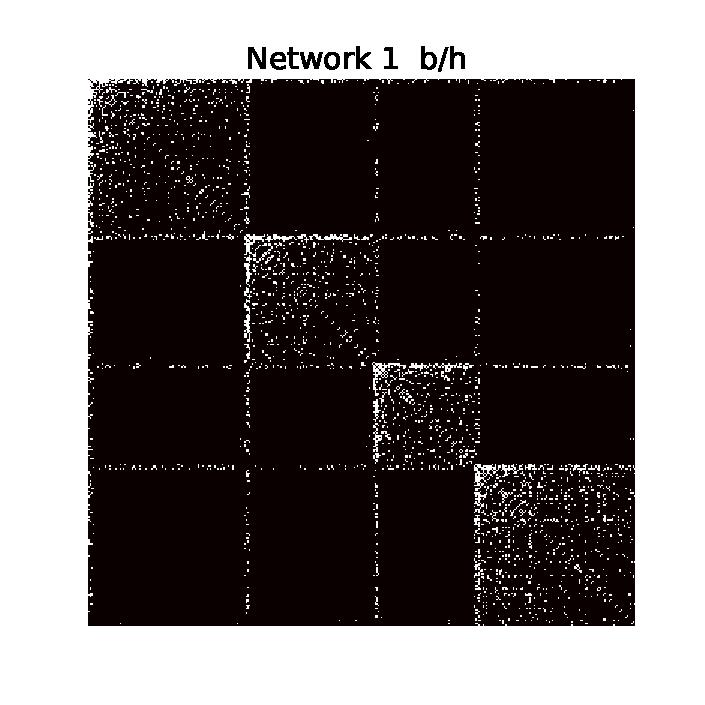
\includegraphics[scale=0.4]{img/g1}
	\endminipage
	\minipage{0.25\textwidth}
	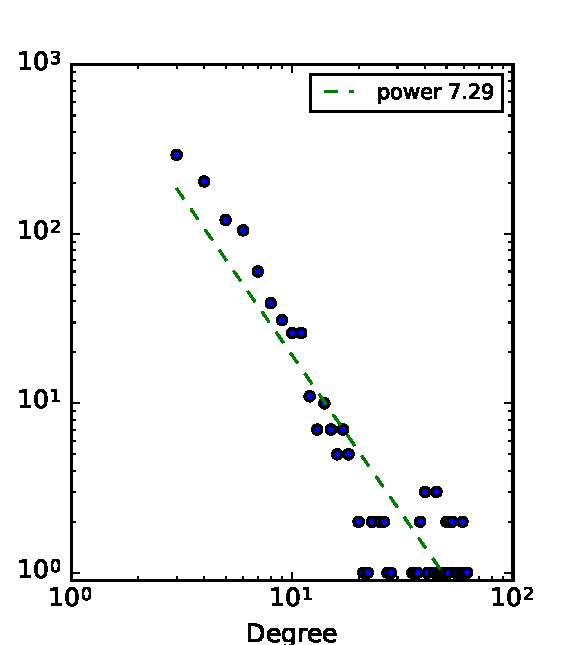
\includegraphics[scale=0.4]{img/g1_d}
	\endminipage
	\vspace{-0.4cm}
	\minipage{0.25\textwidth}
	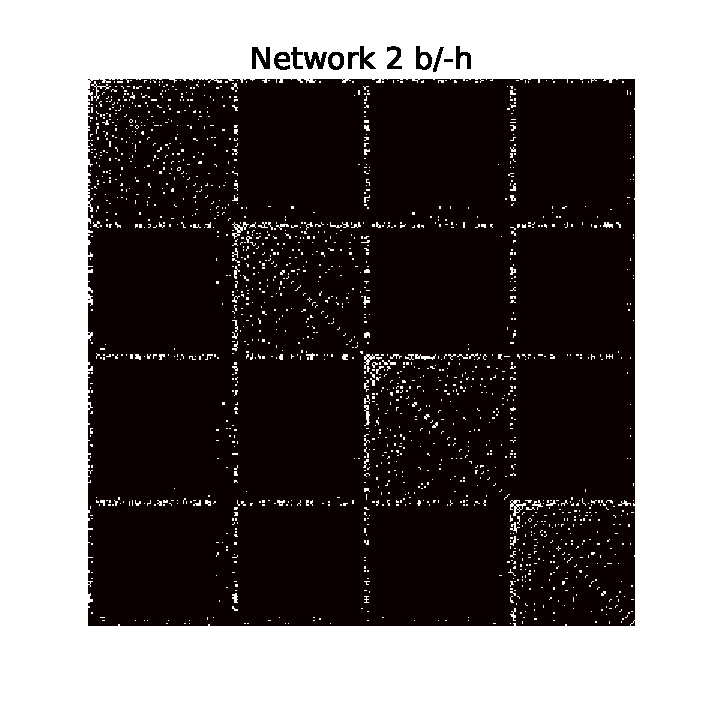
\includegraphics[scale=0.4]{img/g2}
	\endminipage
	\minipage{0.25\textwidth}
	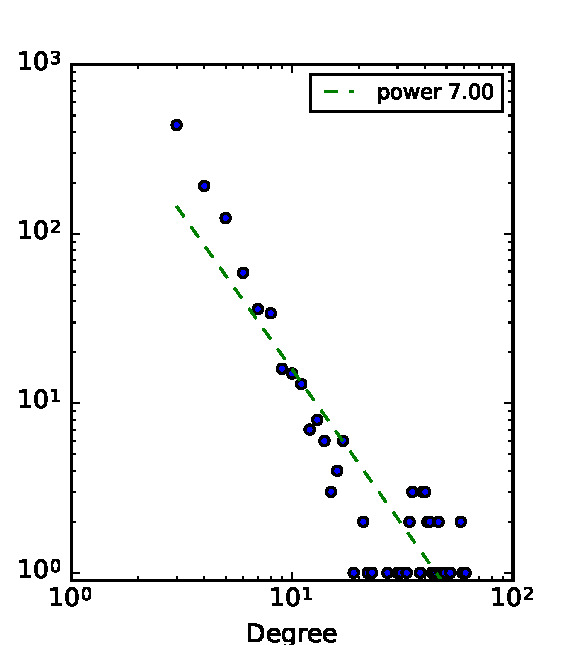
\includegraphics[scale=0.4]{img/g2_d}
	\endminipage
	\vspace{-0.4cm}
	\minipage{0.25\textwidth}
	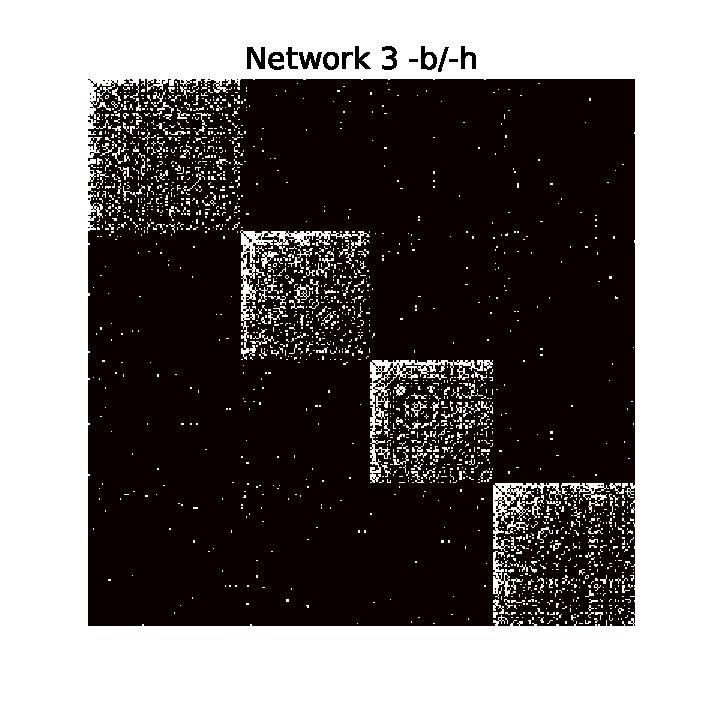
\includegraphics[scale=0.4]{img/g3}
	\endminipage
	\minipage{0.25\textwidth}
	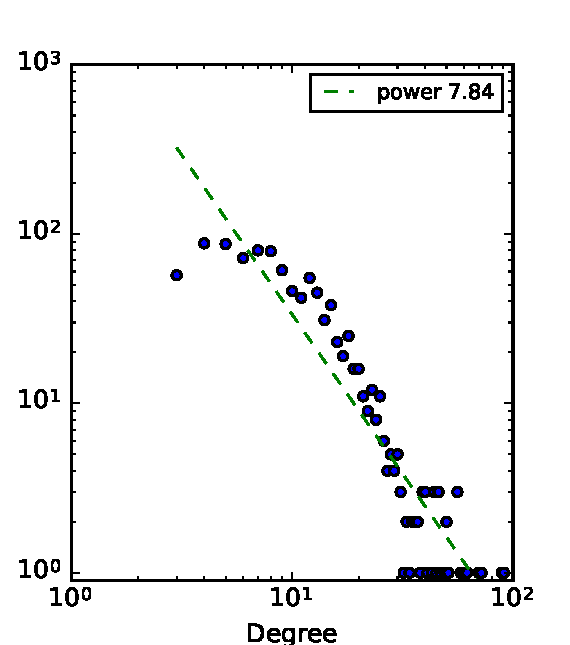
\includegraphics[scale=0.4]{img/g3_d}
	\endminipage
	\vspace{-0.4cm}
	\minipage{0.25\textwidth}
	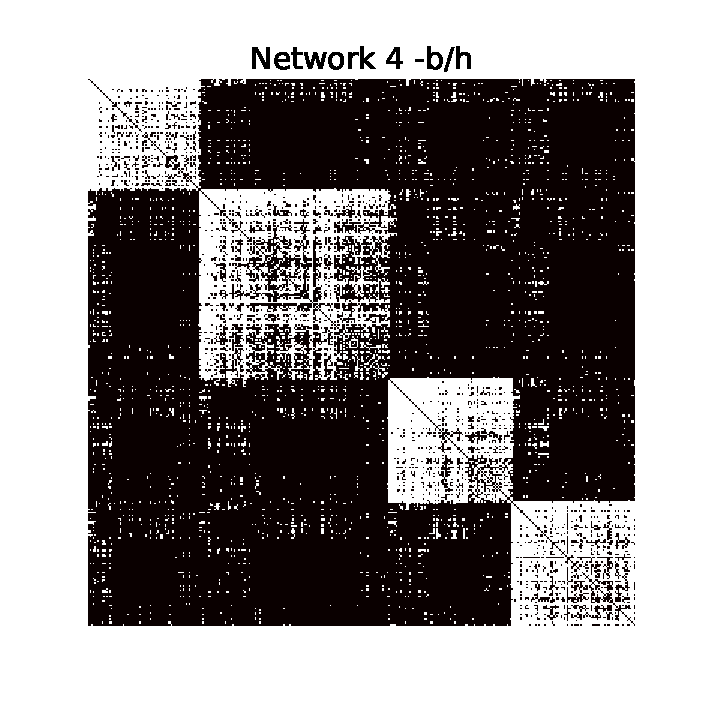
\includegraphics[scale=0.4]{img/g4}
	\endminipage
	\minipage{0.25\textwidth}
	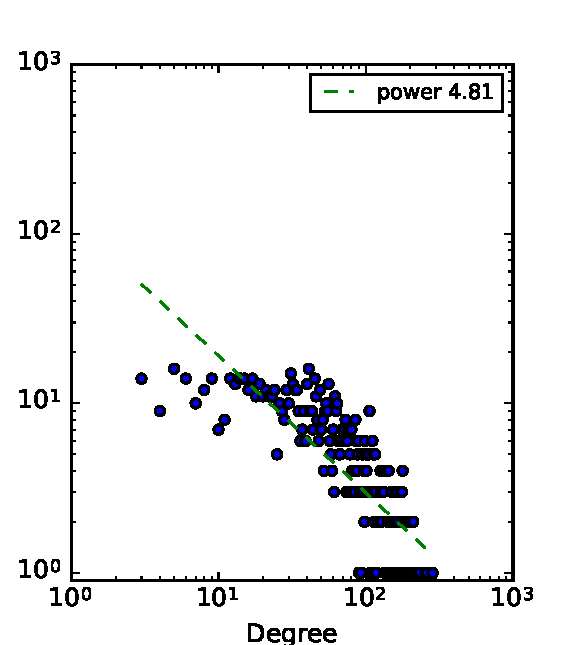
\includegraphics[scale=0.4]{img/g4_d}
	\endminipage
	
	\caption{artificial Networks. (left) adjacency matrix. (right) degree distribution}
	\label{fig:synt_graph}
\end{figure}



\begin{figure}[h]
	\centering
	

	\minipage{0.25\textwidth}
	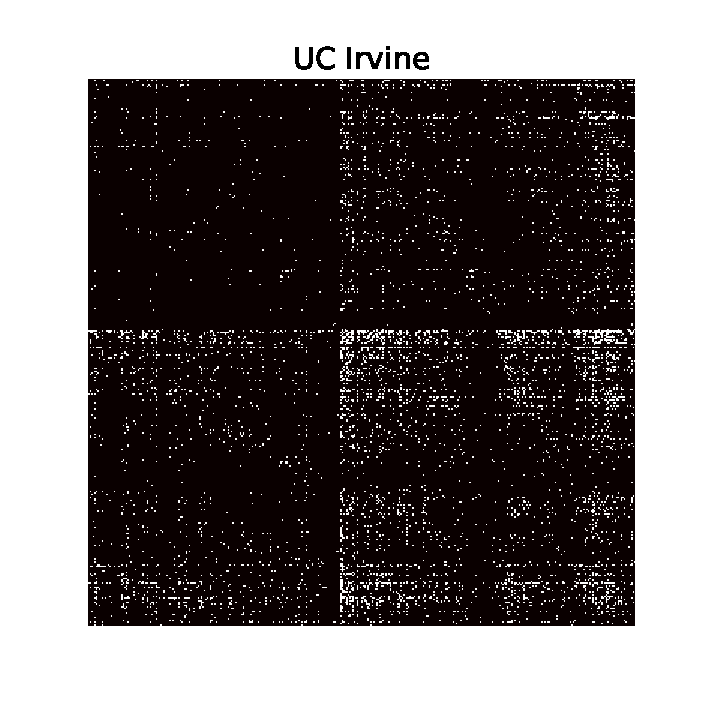
\includegraphics[scale=0.4]{img/irvine}
	\endminipage
	\minipage{0.25\textwidth}
	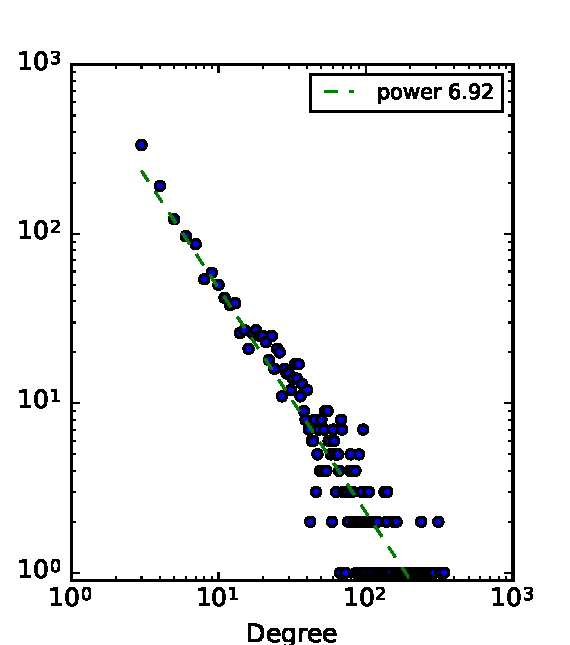
\includegraphics[scale=0.4]{img/irvine_d}
	\endminipage
		\vspace{-0.4cm}
	\minipage{0.25\textwidth}
	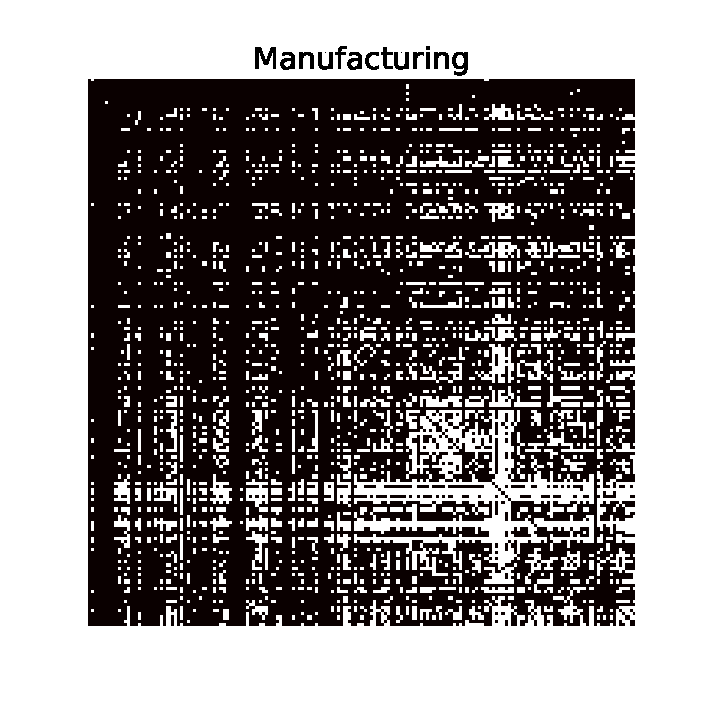
\includegraphics[scale=0.4]{img/manufacturing}
	\endminipage
	\minipage{0.25\textwidth}
	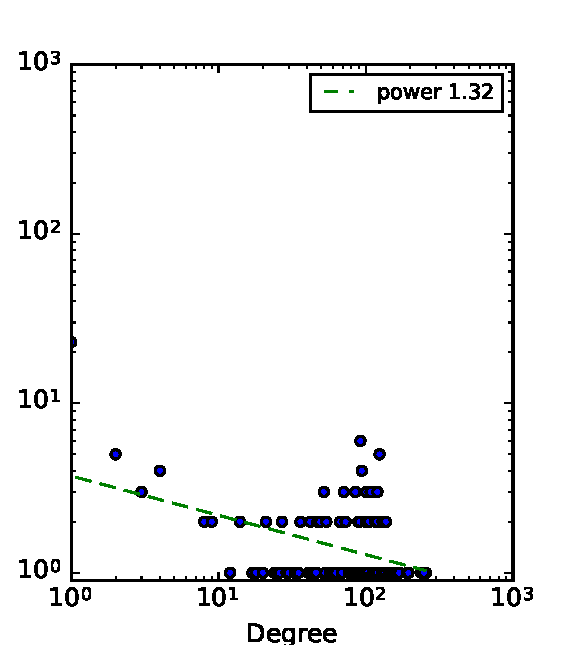
\includegraphics[scale=0.4]{img/manufacturing_d}
	\endminipage
	\caption{Real Networks. (left) adjacency matrix. (right) degree distribution}
	\label{fig:real_graph}
\end{figure}



\subsection{Evaluation Protocol}
For each datasets described,  we run a MCMC inference consisting of 200 iterations to learn the posterior distribution of each the IMMSB model and ILFM, described in \ref{sec:models}. For IMMSB, concentration parameters of HDP were optimized following \cite{HDP} using vague gamma priors $\alpha_0 \sim \text{Gamma}(1,1)$ and $\gamma \sim \text{Gamma}(1,1)$. The parameter for the matrix weights were fixed to $\lambda_0=\lambda_1=0.1$. For ILFM, the IBP hyper-parameter was fixed to $\alpha=0.5$ and the weights hyper-parameter to $\sigma_w = 1$. Each experiences were repeated 10 times, and results were found to be stable regarding on the random initialization and sotchastic optimization.

Our evaluation rely then in two strategy:


\subsubsection{Predictive performance}
We evaluate the performance prediction of the models by building a training set and a testing set from the original datasets. Because the burstiness has a strong impact os the sparsity of the underlying graph, we face a very unbanlanced challenge. Considering this fact, we used two different strategy for building our testing set, in order to assess the impact of the sparsity:

\paragraph{Unbalanced testing set}
We separate our datasets into a training set representing 80 \% of the size of the network, and 20\% for a testing set, randomly chosen. As the dataset has a small density of edges, this testing set ends up with very small amout of edges.

\paragraph{Balanced testing set}
In order to create a balanced testing set, we pick randomly 20 \% of the edges of the network and the same amount of non-links. The testing ends up balanced but it represents a small proportion of the dataset.~\\


We performed a predictive analysis on the testing set and compared the predictive performance of each models with regards to the properties of the network. 
The predictive performance of models is calculated using a traditional precision and recall measures for the predicted links, that we calculated as follows:\\
\begin{align}
    \mathrm{precision}_{V} = Equation precision to complete... \\
    \mathrm{recall}_{V} = Equation recall to complete...
\end{align}


The table \ref{table:unbalanced} and table \ref{table:balanced} respectively shows the overall precision, edge precision and recall results respectively for unbalanced case and tha balance case. Additionnally, the tables show results for several initialization for the number of features $K$ for both models. The last colulmn show the number of latent features to which latent models have converged.

\subsubsection{Generative network}
We consider the generative ability of the models to build new \emph{artificial} networks based on the information learned on the data. This can be expressed by the predictive likelihood given only the hyperparameters $h$ and the training data:
\begin{equation}
    \pr(Y_{new} |Y, h) = \int_{\M} \pr(Y_{new} |Y,\M, h)\pr(\M |, h)d\M
\end{equation}

The generative graph is the expectation of the predective likelihood on the model. The expectation of the generative graph is then given by the bilinear form, according to \ref{MFDCA}:
\begin{equation}
    \E_\M[Y_{new} | Y, \M] = \sigma(F \Phi F^T)
\end{equation}


The figure \ref{fig:gen_graph} shows the mean and variance of the degrees distribution of graphs generated by the ILFM and the IMMSB when fitted on the artificial dataset \ref{sec:datasets}.


\subsection{Results}

\subsubsection{Unbanlanced data}

\paragraph{Results for IMMSB}

For all predictive measure, the overall precision, precision for edge and the recall for edge are better for bursty networks, exept for the Network 4. This is because the density of the latter is higher than the other who make the prediction on this network less inbanlance than the other

On bursty networks, it appears that IMMSB has a tendancy to perform better on the networks where homophily is not strongly present. This can be explain by the fact that IMMSB allows relation between classes, and because strong homophily is correlated to more dense community in the artificial network.


This observation confirm that IMMSB can capture burstiness and slighly better on slighly homophilic network.

\paragraph{Results for ILFM}
Resulst for ILFM show that the models converged to a hihger number of features for networks that are bursty. Even though the number of feature is smaller for the less bursty network, ILFM achive better  results on edge precision an recall.

\paragraph{Comparison of models}
In most case, ILFM performs better than IMMSB but the difference is less significative on bursty networks.

\subsubsection{Balanced data}
\paragraph{Results for IMMSB}

\paragraph{Results for ILFM}
ILFM confirm his tendancy to learn more features on bursty networks. Nevertheless the overall precision and the recall remains significantly better whithin the non-bursty networks. Moreover the overall precision and the recall is significantly better for the strongly homophilic networks.

\paragraph{Comparison of models}


Our results confirm the theoretical analysis on nonparametric models, concerning their affinity to the preferential attachment effect and the homophily effect.

%Our experiments evaluate the preferential attachment and the local preferential attachment on the learned communities trough respectively the distribution of degrees in the networks and inside the communities.

\begin{table} \label{table:real1}
    \caption{IMMSB prediction performance results on real networks, for several feature size initialization.}
\begin{tabular}{lrrrr}
\hline                                                                             
 immsb / mask all   &        5 &       10 &       15 &       20 \\                 
\hline                                                                             
fb\_uc & & & & \\
manufacturing  & & & & \\
\hline                                                                             
\end{tabular}  
\end{table}

\subsubsection{Generative Analisys}

\textcolor{red}{Note about the generative networks: homophily and burstiness measure, respect the theory ?...}
 

\begin{table} \label{table:real2}
    \caption{ILFM predictive performance result on real networks}
\begin{tabular}{lrrrr}
\hline
 ILFM / mask all   &     global &   precision &      recall &   K-\ensuremath{>} \\
\hline
fb\_uc& & & & \\
manufacturing  & & & & \\
\hline
\end{tabular}  
\end{table}

\begin{figure}[h]
	\centering
	
	\minipage{0.25\textwidth}
	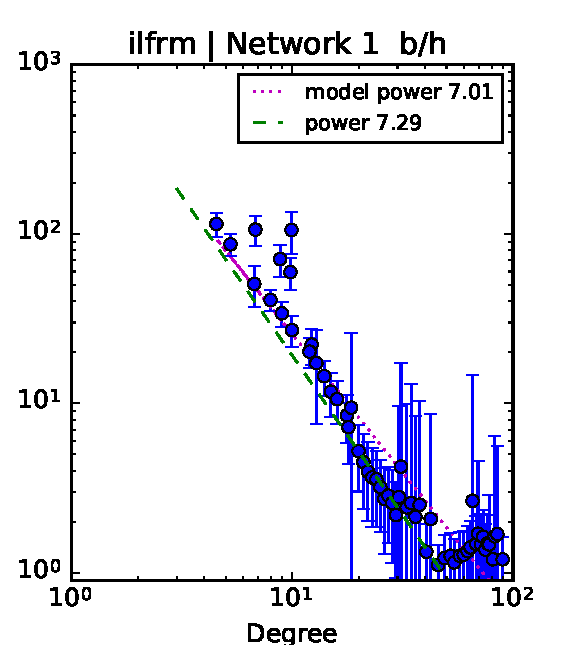
\includegraphics[scale=0.4]{img/ilfrm_g1_d}
	\endminipage
	\minipage{0.25\textwidth}
	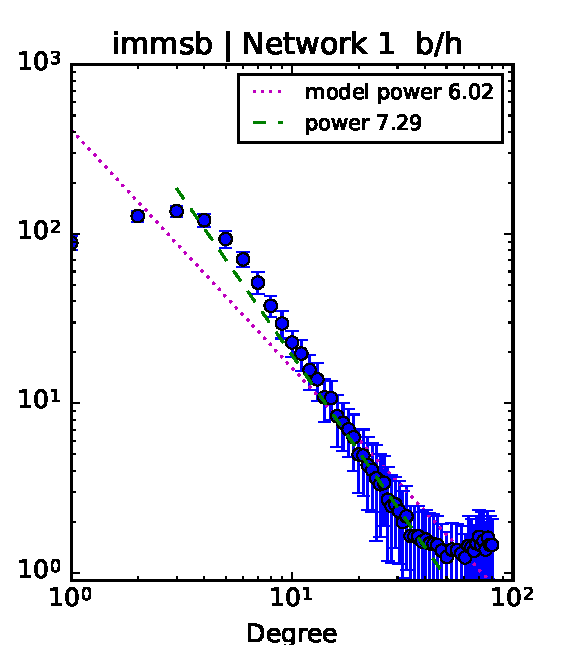
\includegraphics[scale=0.4]{img/immsb_g1_d}
	\endminipage
	\vspace{-0.4cm}
	\minipage{0.25\textwidth}
	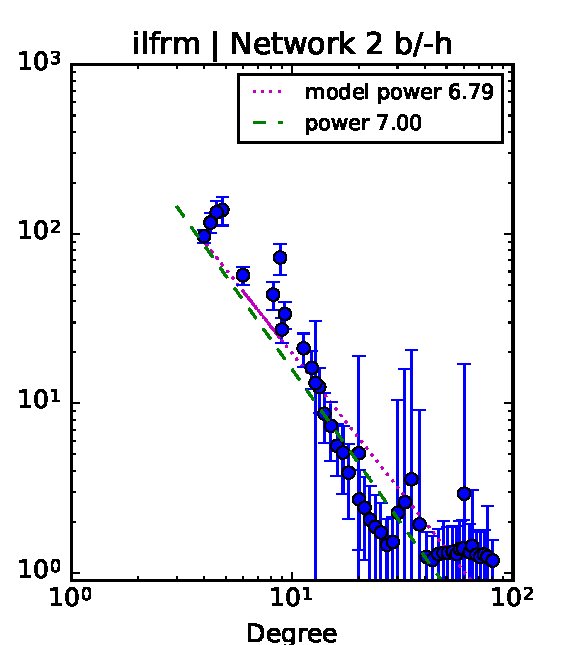
\includegraphics[scale=0.4]{img/ilfrm_g2_d}
	\endminipage
	\minipage{0.25\textwidth}
	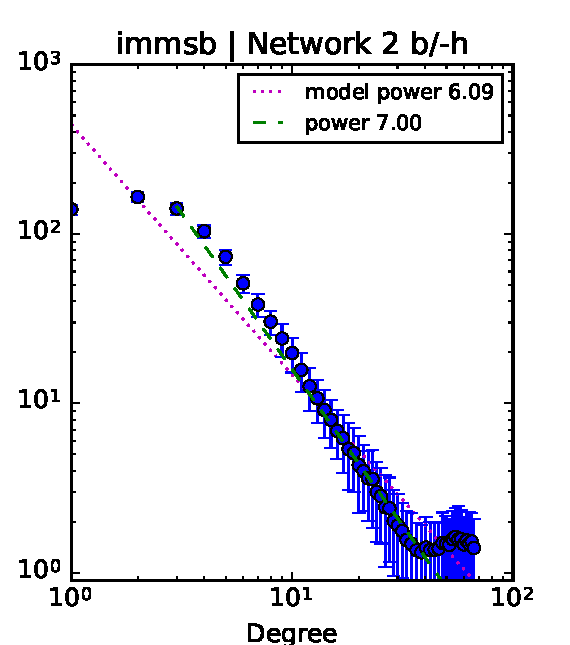
\includegraphics[scale=0.4]{img/immsb_g2_d}
	\endminipage
	\vspace{-0.4cm}
	\minipage{0.25\textwidth}
	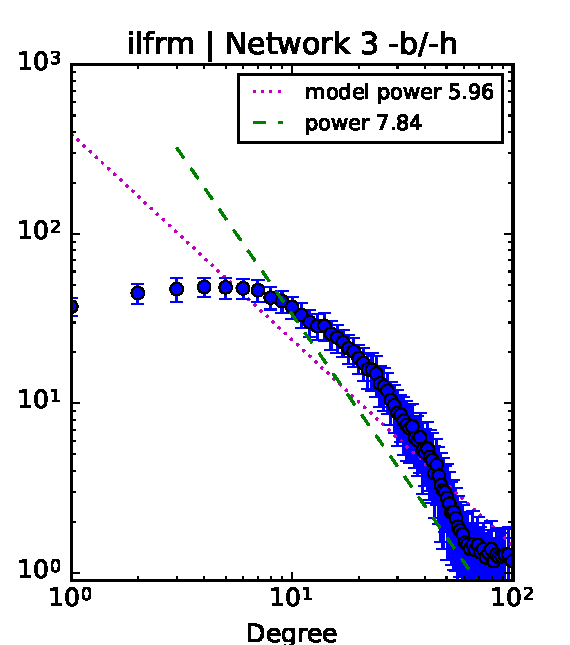
\includegraphics[scale=0.4]{img/ilfrm_g3_d}
	\endminipage
	\minipage{0.25\textwidth}
	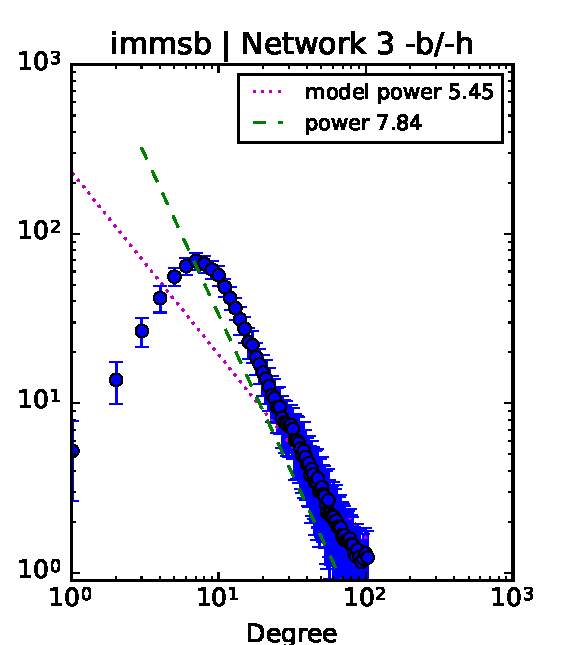
\includegraphics[scale=0.4]{img/immsb_g3_d}
	\endminipage
	\vspace{-0.4cm}
	\minipage{0.25\textwidth}
	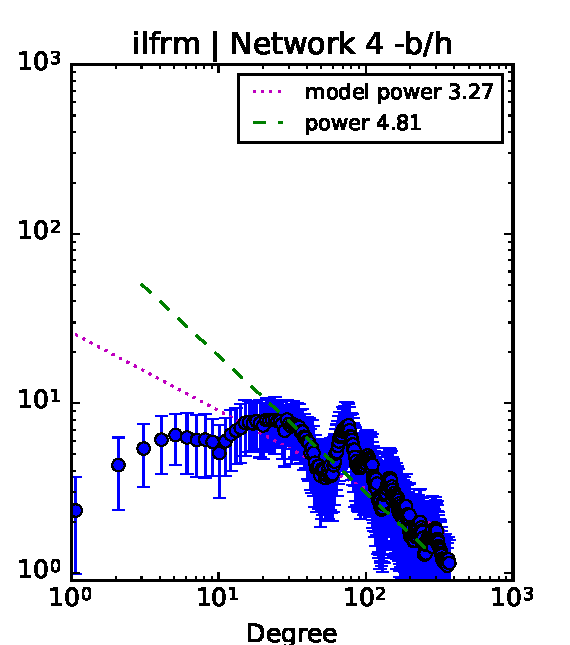
\includegraphics[scale=0.4]{img/ilfrm_g4_d}
	\endminipage
	\minipage{0.25\textwidth}
	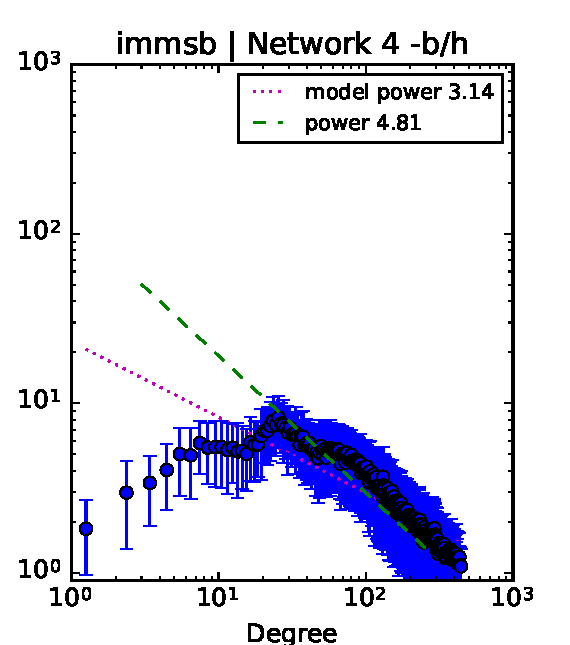
\includegraphics[scale=0.4]{img/immsb_g4_d}
	\endminipage
	
	\caption{Generated Networks with Latent Models learned from artificial datasets}
	\label{fig:gen_graph}
\end{figure}

\begin{figure}[h]
	\centering
	
	\minipage{0.25\textwidth}
	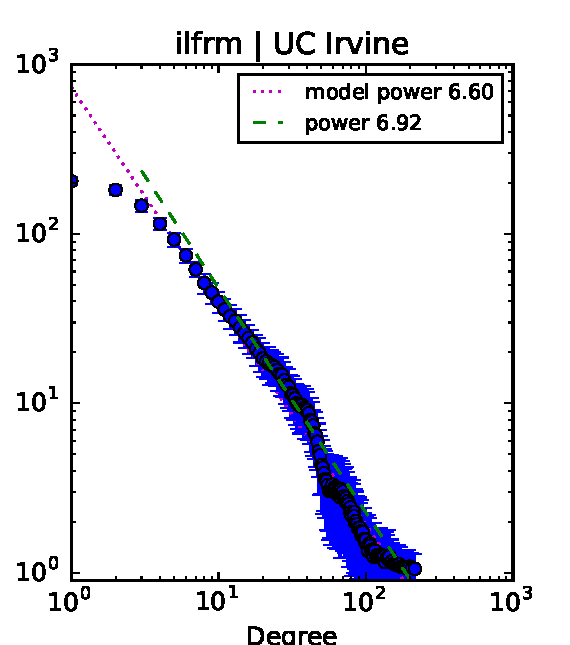
\includegraphics[scale=0.4]{img/ilfrm_irvine_d}
	\endminipage
	\minipage{0.25\textwidth}
	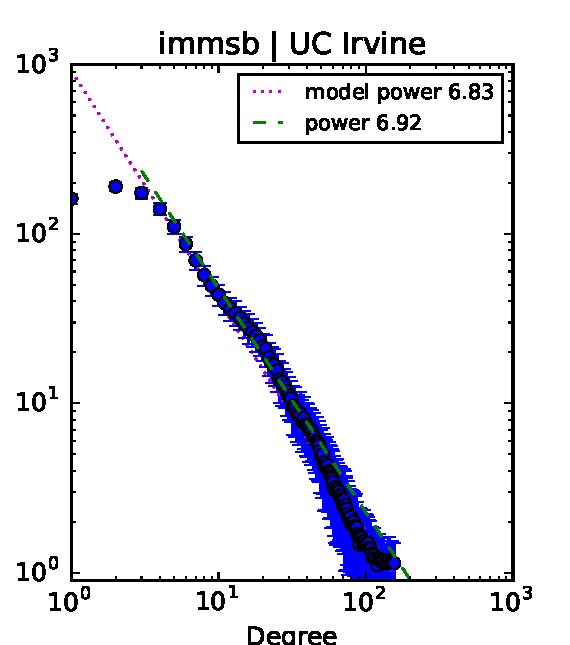
\includegraphics[scale=0.4]{img/immsb_irvine_d}
	\endminipage
	\vspace{-0.4cm}
	\minipage{0.25\textwidth}
	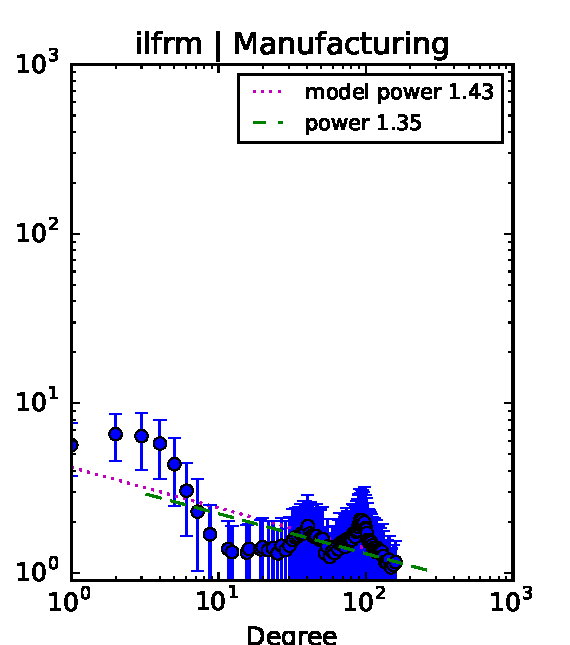
\includegraphics[scale=0.4]{img/ilfrm_manufacturing_d}
	\endminipage
	\minipage{0.25\textwidth}
	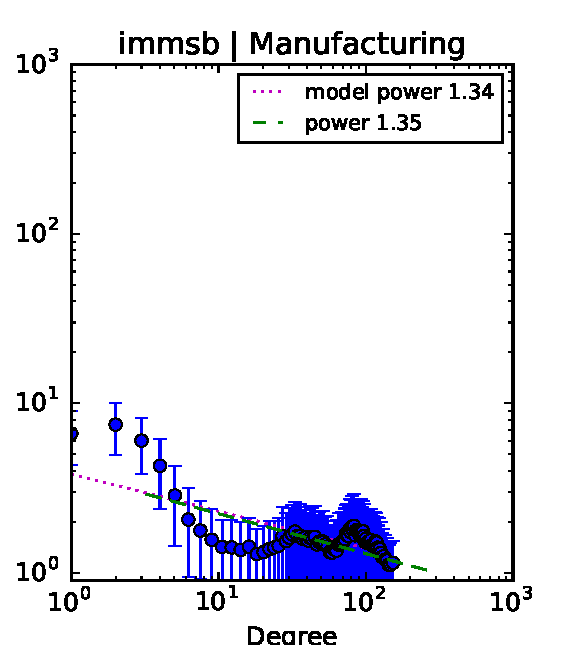
\includegraphics[scale=0.4]{img/immsb_manufacturing_d}
	\endminipage
	
	\caption{Generated Networks with Latent Models learned from artificial datasets}
	\label{fig:gen_graph}
\end{figure}



% Debug 12 / MASK all

% K = 5

\begin{table*}[h] \label{table:unbalanced}
\caption{Predictive Performance on a UnBalanced Testing set}
	\begin{minipage}[h]{0.45\linewidth} 
K = 5\hspace{5pt}
\begin{tabular}{lllll}
\hline
 IMMSB   &   global &   precision &   recall &    K-\ensuremath{>} \\
\hline
 Network1 b/h         &    0.990 &       0.029 &    0.032 & 5.0 $\pm$ 0.0 \\
 Network2 b/-h       &    0.992 &       0.032 &    0.034 & 5.0 $\pm$ 0.0 \\
 Network3 -b/-h       &    0.979 &       0.031 &    0.034 & 5.0 $\pm$ 0.0 \\
 Network4 -b/h       &    0.887 &       0.151 &    0.192 & 5.0 $\pm$ 0.0 \\

\hline
\end{tabular}
\end{minipage}
\hspace{0.8cm}
\begin{minipage}[h]{0.45\linewidth}
\begin{tabular}{lllll}
\hline
  ILFM & global &   precision &   recall &     K-\ensuremath{>} \\
\hline
 Network1 b/h       &    0.990 &       0.051 &    0.053 & 13.4 $\pm$ 0.8    \\
 Network2 b/-h     &    0.992 &       0.044 &    0.045 & 14.0 $\pm$ 2.0    \\
 Network3 -b/-h     &    0.982 &       0.114 &    0.116 & 10.0 $\pm$ 2.1 \\
 Network4 -b/h     &    0.926 &       0.389 &    0.393 & 7.2 $\pm$ 1.6     \\

\hline
\end{tabular}
\end{minipage}

% K = 10

	\begin{minipage}[h]{0.45\linewidth} 
K = 10
\begin{tabular}{lllll}
Network1 b/h         &    0.990 &       0.044 &    0.046 & 10.0 $\pm$ 0.0 \\
 Network2 b/-h       &    0.992 &       0.039 &    0.045 & 10.0 $\pm$ 0.0 \\
 Network3 -b/-h       &    0.979 &       0.030 &    0.035 & 10.0 $\pm$ 0.0 \\
 Network4 -b/h       &    0.897 &       0.202 &    0.238 & 10.0 $\pm$ 0.0 \\

\hline
\end{tabular}
\end{minipage}
\hspace{0.8cm}
\begin{minipage}[h]{0.45\linewidth}
\begin{tabular}{lllll}
 Network1 b/h       &    0.990 &       0.049 &    0.053 & 17.2 $\pm$ 2.8 \\
 Network2 b/-h     &    0.992 &       0.047 &    0.051 & 17.2 $\pm$ 2.1 \\
 Network3 -b/-h     &    0.982 &       0.132 &    0.132 & 12.2 $\pm$ 2.0 \\
 Network4 -b/h     &    0.934 &       0.448 &    0.447 & 9.2 $\pm$ 1.2 \\

\hline
\end{tabular}
\end{minipage}

% K = 15

	\begin{minipage}[h]{0.45\linewidth} 
K = 15
\begin{tabular}{lrrrr}
 Network1 b/h         &    0.990 &       0.038 &    0.041 & 15.0 $\pm$ 0.0 \\
 Network2 b/-h       &    0.992 &       0.036 &    0.038 & 15.0 $\pm$ 0.0 \\
 Network3 -b/-h       &    0.979 &       0.029 &    0.032 & 15.0 $\pm$ 0.0 \\
 Network4 -b/h       &    0.898 &       0.207 &    0.245 & 15.0 $\pm$ 0.0 \\

\hline
\end{tabular}
\end{minipage}
\hspace{0.8cm}
\begin{minipage}[h]{0.45\linewidth}
\begin{tabular}{lrrrr}
 Network1 b/h       &    0.990 &       0.050 &    0.053 & 20.6 $\pm$ 2.1 \\
 Network2 b/-h     &    0.992 &       0.049 &    0.055 & 21.2 $\pm$ 2.1 \\
 Network3 -b/-h     &    0.983 &       0.164 &    0.166 & 17.2 $\pm$ 1.3 \\
 Network4 -b/h     &    0.939 &       0.499 &    0.501 & 14.8 $\pm$ 0.4    \\

\hline
\end{tabular}
\end{minipage}

% K = 20

	\begin{minipage}[h]{0.45\linewidth} 
K = 20
\begin{tabular}{lrrrr}

 Network1 b/h          &   0.9899 &      0.0348 &   0.0375 & 20 \\
 Network2 b/-h       &   0.9923 &      0.0494 &   0.0590 & 20 \\
 Network3 -b/-h      &   0.9794 &      0.0289 &   0.0338 & 20 \\
 Network4 -b/h        &   0.9067 &      0.2646 &   0.3034 & 20 \\
\hline
\end{tabular}
\end{minipage}
\hspace{0.8cm}
\begin{minipage}[h]{0.45\linewidth}
\begin{tabular}{lrrrr}
Network1 b/h       &   0.9902 &      0.0641 &   0.0626 &  23 \\
Network2 b/-h     &   0.9915 &      0.0477 &   0.0636 & 17 \\
Network3 -b/-h     &   0.9827 &      0.1523 &   0.1518 &  20 \\
Network4 -b/h     &   0.9396 &      0.4986 &   0.5053 &  22 \\
\hline
\end{tabular}
\end{minipage}
\end{table*}


%%%%%%%%%%%%%%%%%%%%%%%%%%%%%%%%%%%%%%%%%%%%%%%%%%%%%%%%%%%%%%%%%%%%
%%%%%%%%%%%%%%%%%%%%%%%%%%%%%%%%%%%%%%%%%%%%%%%%%%%%%%%%%%%%%%%%%%%%
%%%%%%%%%%%%%%%%%%%%%%%%%%%%%%%%%%%%%%%%%%%%%%%%%%%%%%%%%%%%%%%%%%%%
%%%%%%%%%%%%%%%%%%%%%%%%%%%%%%%%%%%%%%%%%%%%%%%%%%%%%%%%%%%%%%%%%%%%
%%%%%%%%%%%%%%%%%%%%%%%%%%%%%%%%%%%%%%%%%%%%%%%%%%%%%%%%%%%%%%%%%%%%
%%%%%%%%%%%%%%%%%%%%%%%%%%%%%%%%%%%%%%%%%%%%%%%%%%%%%%%%%%%%%%%%%%%%


% Debug 11 / MASK 1

% K = 5

\begin{table*}[h] \label{table:balanced}
\caption{Predictive Performance on a Balanced Testing set}
	\begin{minipage}[h]{0.45\linewidth} 
K =  5\hspace{5pt}
\begin{tabular}{lrlll}
\hline
 IMMSB   &   global &   precision &   recall &    K-\ensuremath{>} \\
\hline
 Network1 b/h          &    0.549 &       0.758 &    0.022 & 5.0 $\pm$ 0.0 \\
 Network2 b/-h        &    0.558 &       0.834 &    0.019 & 5.0 $\pm$ 0.0 \\
 Network3 -b/-h        &    0.527 &       0.729 &    0.027 & 5.0 $\pm$ 0.0 \\
 Network4 -b/h        &    0.557 &       0.743 &    0.162 & 5.0 $\pm$ 0.0 \\

\hline
\end{tabular}
\end{minipage}
\hspace{0.8cm}
\begin{minipage}[h]{0.45\linewidth}
\begin{tabular}{lrlll}
\hline
 ILFM   &   global &   precision &   recall &     K-\ensuremath{>} \\
\hline
 Network1 b/h        &    0.568 &       0.912 &    0.047 & 13.6 $\pm$ 2.3 \\
 Network2 b/-h      &    0.574 &       0.893 &    0.041 & 16.4 $\pm$ 3.4 \\
 Network3 -b/-h      &    0.571 &       0.912 &    0.100 & 9.2 $\pm$ 1.3 \\
 Network4 -b/h      &    0.668 &       0.906 &    0.362 & 7.6 $\pm$ 1.3 \\

\hline
\end{tabular}
\end{minipage}

% K = 10

	\begin{minipage}[h]{0.45\linewidth} 
K = 10
\begin{tabular}{lrrrr}
 Network1 b/h          &    0.558 &       0.842 &    0.028 & 10.0 $\pm$ 0.0 \\
 Network2 b/-h        &    0.567 &       0.926 &    0.034 & 10.0 $\pm$ 0.0 \\
 Network3 -b/-h        &    0.530 &       0.776 &    0.027 & 10.0 $\pm$ 0.0 \\
 Network4 -b/h        &    0.567 &       0.764 &    0.184 & 10.0 $\pm$ 0.0 \\

\hline
\end{tabular}
\end{minipage}
\hspace{0.8cm}
\begin{minipage}[h]{0.45\linewidth}
\begin{tabular}{lrrrr}
 Network1 b/h        &    0.556 &       0.928 &    0.044 & 17.2 $\pm$ 2.0 \\
 Network2 b/-h      &    0.573 &       0.935 &    0.041 & 17.6 $\pm$ 3.2    \\
 Network3 -b/-h      &    0.579 &       0.947 &    0.118 & 12.8 $\pm$ 0.9 \\
 Network4 -b/h      &    0.718 &       0.943 &    0.457 & 10.8 $\pm$ 0.7 \\

\hline
\end{tabular}
\end{minipage}

% K = 15

	\begin{minipage}[h]{0.45\linewidth} 
K = 15
\begin{tabular}{lrrrr}
 Network1 b/h          &    0.555 &       0.871 &    0.035 & 15.0 $\pm$ 0.0 \\
 Network2 b/-h        &    0.570 &       0.854 &    0.030 & 15.0 $\pm$ 0.0 \\
 Network3 -b/-h        &    0.532 &       0.728 &    0.027 & 15.0 $\pm$ 0.0 \\
 Network4 -b/h        &    0.565 &       0.757 &    0.178 & 15.0 $\pm$ 0.0 \\

\hline
\end{tabular}
\end{minipage}
\hspace{0.8cm}
\begin{minipage}[h]{0.45\linewidth}
\begin{tabular}{lrrrr}
 Network1 b/h        &    0.569 &       0.928 &    0.046 & 20.8 $\pm$ 1.3 \\
 Network2 b/-h      &    0.564 &       0.903 &    0.042 & 21.6 $\pm$ 2.4 \\
 Network3 -b/-h      &    0.594 &       0.952 &    0.153 & 18.0 $\pm$ 0.8 \\
 Network4 -b/h      &    0.723 &       0.945 &    0.467 & 15.0 $\pm$ 0.0    \\

\hline
\end{tabular}
\end{minipage}

% K = 20

	\begin{minipage}[h]{0.45\linewidth} 
K = 20
\begin{tabular}{lrrrr}

 Network1 b/h           &   0.5501 &      0.8980 &   0.0425 & 20 \\
 Network2 b/-h        &   0.5734 &      0.9615 &   0.0326 & 20 \\
 Network3 -b/-h       &   0.5286 &      0.6456 &   0.0255 & 20 \\
 Network4 -b/h         &   0.5577 &      0.7475 &   0.1662 & 20 \\
\hline
\end{tabular}
\end{minipage}
\hspace{0.8cm}
\begin{minipage}[h]{0.45\linewidth}
\begin{tabular}{lrrrr}
 Network1 b/h         &   0.5428 &      0.9737 &   0.0359 &  21 \\
 Network2 b/-h      &   0.5577 &      0.8462 &   0.0389 &  20 \\
 Network3 -b/-h     &   0.5997 &      0.9503 &   0.1630 &  22 \\
 Network4 -b/h      &   0.7291 &      0.9473 &   0.4813 & 20 \\
\hline
\end{tabular}
\end{minipage}
\end{table*}


\begin{table}
    \caption{Homohily test for IMMSB fit on diferent configarations}
\begin{tabular}{lrrrr}
\hline
IMMSB / Balanced   &     5 &    10 &    15 &    20 \\
\hline
Network 1 b/h          & 0.066 & 0.100 & 0.109 & 0.127 \\
Network 2 b/-h        & 0.065 & 0.100 & 0.141 & 0.126 \\
Network 3 -b/-h       & 0.035 & 0.083 & 0.067 & 0.076 \\
Network 4 -b/h         & 0.421 & 0.450 & 0.460 & 0.460 \\
\hline
\end{tabular}
\end{table}

\begin{table}
    \caption{Homohily test for ILFM fit on different configurations}
\begin{tabular}{lrrrr}
\hline
ILFM / Balanced   &     5 &    10 &    15 &    20 \\
\hline
Network 1 b/h        & 0.010 & 0.140 & 0.128 & 0.223 \\
Network 2 b/-h      & 0.097 & 0.079 & 0.245 & 0.147 \\
Network 3 -b/-h     & 0.037 & 0.084 & 0.131 & 0.184 \\
Network 4 -b/h       & 0.181 & 0.442 & 0.479 & 0.503 \\
\hline
\end{tabular}
\end{table}



\section{Related Work}

%Burstiness on topic model:
%Modeling Word Burstiness Using the Dirichlet Distribution (DCM)
%Accounting for Burstiness in Topic Models (DCMLDA)
%Proposal of a-MMSB in : Scalable Inference of Overlapping Communities with high diagonal only...

%to read: Stochastic blockmodels and community structure in networks


\section{Conclusion}
\label{sec:concl}

%%% Conclusion on the paper
This work introduce a framework which aims at studying topological properties on social networks by giving definition which are consistent with the Bayesian framework. Using this framework, We show that strong relation exist between major relational latent model and fundamental properties of networks, the preferential attachment effect and the homophily effect.~\\ 

%%% Perspectives
This work offers many perspectives to improve our understanding of Bayesian relational models for complex networks. Obviously, our implementation based on MCMC inference does not allow us to scale to large networks. We will focus in the future in implementing variational inference scheme to be able to validate our theoretical results on much larger real networks. An other direction is to study the impact of hyperparameters on the structure of the generative network. Particularly a more well adapted optimization for nonparametric models could lead to a better control for capturing the preferential attachment effect. Especially by generalizing both the IBP and the HDP prior to their general counterpart, the 2-parameters IBP and the Pitman Yor Process. To conclude on perspective, it worth to mention that complex networks include other important properties of networks to study, such as the small world effect and the temporal dynamics of the network topology.

%\input{sup.tex}

\bibliographystyle{unsrt}
\bibliography{./a}

\appendix
\section{Appendix}
\label{sec:append}

\subsection{Mixed membership Models}
\label{sec:mixmembership}
In the Mixed Membership Models \cite{MMM}, the models can be defined at the link level by the likelihood of generating a link between two nodes given the contribution of each classes (or features). For IMMSB, this likelihood is straightforward, but for ILFM the class membership is defined deterministically by the binary vector $\mat{f}$. If the $k^{th}$ row is active (equal to one) then the node has the membership, else it doesn't. Hence for ILFM, We can write the likelihood  using the Dirac distribution $\delta(x)$ that gives one for $x=0$ as follows:

\begin{align}
    \pr(y_{ij} \mid \mat{F}, \mat{\Phi } ) &= \sigma \sum_{k, k'} \pr(y_{ij}\mid\phi_{k,k'}) \pr(k \mid \mat{f}_i) \pr(k' \mid \mat{f}_j) \\
    &=  \sigma \sum_{k, k'} \phi_{k,k'}  \delta(1-f_{ik}) \delta(1-f_{jk'})
    \end{align}
    

\subsection{Collapsed Gibbs sampling updates for IMMSB}

We provide here the derivation of the updates of the IMMSB model, described in Section~\ref{sec:models}.

%From the definition of the model, one has: $\pr(z_{ij} = k \mid \mat{f}_i) = f_{ik}$.

%\textcolor{red}{Adrien, peux-tu donner la d\'erivation ? La forme actuelle n'est valable que pour MMSB.} 

%heeeere \alpha is \alpha_0

Inference for the IMMSB model by using the Collapse Gibbs sampler gives updates for class assignment $Z \in N\times N \times 2$ for each interactions $Y \in N\times N$. Thus for all pair of interaction (i,j) we jointly sample the classes $(z_{ij}, z_{ji})$ who implicitly, take the values $(k,k')$ :
\begin{align} \label{eq:cgs}
&\pr(z_{ij}, z_{ji} \mid Z^-, Y,  \mat{\beta}, \alpha, \mat{\lambda} )  \\
&\propto\pr(z_{ij}, z_{ji} \mid Z^-, \alpha,\mat{\beta}) \pr(y_{ij} \mid Y^{-ij},  Z^-,z_{ij}, z_{ji},  \mat{\lambda} ) \nonumber
\end{align}
The term $Z^-$ denote that both $z_{ij}$ and $z_{ji}$ are exclude from $Z$. We now treat the first term of equation \ref{eq:cgs}.  
\begin{align}
&\pr(z_{ij}, z_{ji} \mid Z^-, \alpha,\mat{\beta})\\
&\propto \pr(z_{i\rightarrow j} \mid \{z_{i\rightarrow j'}\}_{j'\neq j}, \{z_{j'\leftarrow i}\}_{j'=1}^N, \alpha,\mat{\beta}) \\
& \quad .  \pr(z_{i\leftarrow j} \mid \{z_{i'\leftarrow j}\}_{i'\neq i}, \{z_{j\leftarrow i'}\}_{i'=1}^N, \alpha,\mat{\beta}) \nonumber
\end{align}
Let's consider the density of $z_{i\rightarrow j}$:
\begin{align}
&\propto \pr(z_{i\rightarrow j} \mid \{z_{i\rightarrow j'}\}_{j'\neq j}, \{z_{j'\leftarrow i}\}_{j'=1}^N, \alpha,\mat{\beta})  \\
&\propto \int_{f_i} \pr(f_i \mid \mat{\beta}, \alpha) \pr(z_{ij} \mid f_i) \prod_{j'\neq j} \pr(z_{ij'} \mid f_i) \prod_{j' =  1}^N  \pr(z_{j' i} \mid f_i)  df_i \nonumber
\end{align}


Due to the an augmented representation of the Chinese Restaurant Franchise (CRF) with the Stick Breaking Process \cite{HDP}, the density of the features can be approximated by the following Dirichlet distribution;
\begin{equation}
f_i \mid \mat{\beta}, \alpha \sim Dir(\alpha \beta_1,..,\alpha\beta_K, \alpha\beta_{new})
\end{equation}
Where $\alpha\beta_{new}$ represent the contribution for sampling a new class. Since $\pr(z_{ij} \mid f_i)$ is drawn from a multinomial, the model is said to be conjugate and reduce to a simple closed form expression:
\begin{enumerate}
\item If the class $k$ has already been observed:
   \begin{align}
    \pr(z_{ij} =k \mid .) &\propto N_{ik}^{-ij} + \alpha_0 \beta_k
    \label{eq:update-immsb}
   \end{align}
\item In case of a new class $k_{new}$:
   \begin{align}
    \pr(z_{ij} =k_{new} \mid.) &\propto \alpha_0 \beta_{new} \nonumber   
   \end{align}
\end{enumerate}
 Where  $N_{ik}$ is the count for node $i$ being assigned to class $k$. As we show that the equations are symmetric, sampling for $z_{ji}$ is straightforward.

~\\
Again, referring the CRF, the sampling of the tables configuration $\mat{m}$ is given by: 
\begin{equation}
\pr(m_{ik} \mid Z, \bm{m}^{-ik}, \mat{\beta} ) = \frac{\Gamma(\alpha_0 \beta_k)}{\Gamma(\alpha_0 \beta_k + n_{j\bm{.   }k})} s(n_{j\bm{.}k}, m) (\alpha_0 \beta_k)^m
\end{equation}
And, finnaly  $\mat{\beta}$ is obtained by:
\begin{equation}
\mat{\beta} \sim Dir(m_1,.., m_K, \gamma)  
\end{equation}
Where $s(n,m)$ is the unsigned Stirling number of the first kind.


~\\
Finally, when the markov chain reach the stationnary distribution, the models parameters $\M = \{\mat{\Phi}, \mat{F}\}$ can be recovered by averaging the topics assignement counts for each membership and each relation:
\begin{align}
&\pr(f_{ik}) =\frac{ N_{ik} + \alpha\beta_k}{ N_{i\bm{.}} + \sum_k\alpha_k }\\
&\pr(\phi_c ) = \frac{M_{c1} + \lambda_1}{M_{c\bm{.}} + \lambda_0 + \lambda_1}
\end{align}


The count for node $i$ being assigned to membership $k$ is $N_{ik}$. And the count of for all couple of classes $c=(k,k')$ being associated to relation $r$ is $M_{cr}$. Note that in our case, the relation $r$ take values in (0,1) accounting for link or non-link between two node.


\end{document}

\grid
